%%
%% Wahrscheinlichkeit & Statistik, FS 2018
%%
%% (C) 2018 Jens Eirik Saethre
%% 
%% Licence: Creative Commons Attribution-Share Alike 3.0 Unported
%% http://creativecommons.org/licenses/by-sa/3.0/
%% 

\documentclass[11pt]{article}
\usepackage[left=1mm, right=1mm, top=1mm, bottom=1mm,paperwidth=140mm, paperheight=297mm]{geometry}
\usepackage[utf8x]{inputenc}
\usepackage{amssymb, amsfonts, amsmath}
\usepackage{xcolor}
\usepackage[e]{esvect}
\usepackage{floatrow} % allows to insert pictures into proofs and theorems

\usepackage{cancel}

\usepackage{graphicx}
%\usepackage{picins}
\usepackage{tabularx}
\usepackage{mwe} % for blindtext and example-image-a in example
\usepackage{wrapfig}
\usepackage{framed}
\usepackage{booktabs}
\colorlet{shadecolor}{orange!15}

\usepackage{multirow}
\usepackage{multicol}
\columnsep24pt
\columnseprule0.1pt

% use greek letters for phi and epsilon
\renewcommand{\phi}{\varphi}
\renewcommand{\epsilon}{\varepsilon}

% bolds math symbols
\newcommand{\bs}{\boldsymbol}
% Shortcut to write caligraphic math symbols
\newcommand{\mc}{\mathcal}
% norm
\newcommand{\norm}[1]{\left| \!\:\! \left| #1 \right| \!\:\! \right|}

% some shortcuts
\newcommand{\ds}{\displaystyle}
\newcommand{\arr}{\rightarrow}
\newcommand{\Arr}{\Rightarrow}
\newcommand{\LRA}{\Leftrightarrow}
\newcommand{\LLRA}{\Longleftrightarrow}
\newcommand{\nop}[1]{}
\newcommand{\rank}{\operatorname{rank}}
\newcommand{\cond}{\operatorname{cond}}
\newcommand{\grad}{\operatorname{grad}}
\newcommand{\argmin}{\mathop{\mathrm{argmin}}}
\newcommand{\argmax}{\mathop{\mathrm{argmax}}}
\newcommand{\mx}{\mathop{\mathrm{max}}}
\newcommand{\bigcupdot}{\bigcup \hspace{-0.35cm} \cdot}


% stuff for integrals
\newcommand{\intl}{\int\limits}
\newcommand{\rmd}{\mathrm{d}}
\newcommand{\rmD}{\mathrm{D}}

% number sets
\newcommand{\R}{\mathbb{R}}
\newcommand{\E}{\mathbb{E}}
\newcommand{\Z}{\mathbb{Z}}
\newcommand{\N}{\mathbb{N}}
\newcommand{\Q}{\mathbb{Q}}
\newcommand{\C}{\mathbb{C}}
\newcommand{\K}{\mathbb{K}}
\newcommand{\M}{\mathbb{M}}

% big-o notation
\newcommand{\bigO}{\mathcal{O}}

% 'with' in set notation
\newcommand{\with}{\;|\;}

% hyperref
\usepackage[colorlinks=false,pdfborder = {0 0 0 0}]{hyperref}


\parindent0pt
\setcounter{secnumdepth}{4}

%% Redefine the \paragraph command:
\makeatletter
\renewcommand\paragraph{\@startsection{paragraph}{4}{0mm}%
	{-\baselineskip}%
	{0.5\baselineskip}%
	{\normalfont\bfseries}%
}%
\makeatother 

% algorithms
\usepackage{algorithmic}
\usepackage{algorithm}
\algsetup{linenodelimiter=}

% listings
\definecolor{darkgreen}{RGB}{0,127,14}
\definecolor{purple}{RGB}{75,0,130}
\usepackage{listings}


\usepackage{listings}
\usepackage{xcolor}
\lstset { %
    language=Pascal,
    backgroundcolor=\color{black!5}, % set backgroundcolor
    basicstyle=\footnotesize,% basic font setting
    escapeinside={!}{!},
    tabsize=2,
}

\def\doubleunderline#1{\underline{\underline{#1}}}

% theorem package
\usepackage{amsthm}
\usepackage{thmtools}
\newtheoremstyle{my-thm-style}% name
{6pt}% Space above
{5pt}% Space below
{}% Body font
{}% Indent amount
{\bfseries}% Theorem head font
{}% Punctuation after theorem head
{8pt}% Space after theorem head
{}% Theorem head spec (can be left empty, meaning `normal')

\definecolor{orange}{rgb}{1,0.5,0}
\definecolor{blue}{RGB}{135,206,250}

\declaretheoremstyle[
headfont=\normalfont\bfseries,
notefont=\mdseries, notebraces={(}{)},
bodyfont=\normalfont,
postheadspace=8pt,
spaceabove=1pt,
mdframed={
  skipabove=2pt,
  skipbelow=2pt,
  hidealllines=false,
  backgroundcolor={orange!15},
  innerleftmargin=2pt,
  innerrightmargin=2pt}
]{def}

\declaretheoremstyle[
headfont=\normalfont\bfseries,
notefont=\mdseries, notebraces={(}{)},
bodyfont=\normalfont,
postheadspace=8pt,
spaceabove=1pt,
mdframed={
  skipabove=2pt,
  skipbelow=2pt,
  hidealllines=false,
  backgroundcolor={purple!10},
  innerleftmargin=2pt,
  innerrightmargin=2pt}
]{sat}

\declaretheoremstyle[
headfont=\normalfont\bfseries,
notefont=\mdseries, notebraces={(}{)},
bodyfont=\normalfont,
postheadspace=8pt,
spaceabove=1pt,
mdframed={
  skipabove=2pt,
  skipbelow=2pt,
  hidealllines=false,
  backgroundcolor={green!10},
  innerleftmargin=2pt,
  innerrightmargin=2pt}
]{lem}

\declaretheoremstyle[
headfont=\normalfont\bfseries,
notefont=\mdseries, notebraces={(}{)},
bodyfont=\normalfont,
postheadspace=8pt,
spaceabove=1pt,
mdframed={
  skipabove=2pt,
  skipbelow=2pt,
  hidealllines=false,
  backgroundcolor={green!0},
  innerleftmargin=2pt,
  innerrightmargin=2pt}
]{kor}

\declaretheorem[style=def, name=Def. , numberwithin=section]{definition}
\declaretheorem[style=sat, name=Satz, numberwithin=section]{satz}
\declaretheorem[style=lem, name=Lemma, numberwithin=section]{lemma}
\declaretheorem[style=kor, name=Korollar, numberwithin=section]{korollar}


\usepackage[english,german]{babel} 
\begin{document}


\author{Jens Eirik Saethre}
\title{Wahrscheinlichkeit \& Statistik}

\date{\today}
%\maketitle

\setcounter{tocdepth}{2}
%\tableofcontents

%\thispagestyle{empty}
%\newpage
\setcounter{page}{1}

%\begin{multicols}{2}

% include the individual chapters
\part{Wahrscheinlichkeitstheorie}
\setcounter{section}{0} % not strictly necessary, but sometimes useful

\section{Wahrscheinlichkeitenfffff}

\subsection{Grundbegriffe}
\begin{definition}[\textbf{Ereignisraum}]
\textit{Ereignisraum} oder \textit{Grundraum} $\bs{\Omega} \neq \emptyset$ ist Menge aller möglichen Ergebnisse des Zufallsexperiments. Seine Elemente $w\in \Omega$ heissen \textit{Elementarereignisse}.
\end{definition} 

\begin{definition}[\textbf{Potenzmenge, Ereignis}]
Die \textit{Potenzmenge} von $\Omega$ wird mit $2^\Omega$ oder mit $\mathcal{P}(\Omega)$ bezeichnet und ist die Menge aller Teilmengen von $\Omega$. Ein \textit{Ereignis} ist ein solches Element der Potenzmenge, also $A\in\mathcal{P}(\Omega)$. Die Klasse aller beobachtbaren Ereignisse ist $\mathcal{F}$, ebenfalls eine Teilmenge der Potenzmenge.
\end{definition}

\begin{definition}[$\bs{\sigma}$\textbf{-Algebra}]
Ein Mengensystem $\mathcal{F}$ ist eine $\sigma$-Algebra, falls
\begin{itemize}
\item[(i)] $\Omega \in \mathcal{F}$
\item[(ii)] für jedes $A\in\mathcal{F}$ ist auch Komplement $A^\complement \in \mathcal{F}$. 
\item[(iii)] für jede Folge $(A_n)_{n\in\N}$ mit $A_n \in \mathcal{F}$ für alle $n\in \N$ ist auch $\bigcup_{n=1}^\infty A_n \in \mathcal{F}$.
\end{itemize}
\end{definition}

\begin{definition}[\textbf{Wahrscheinlichkeitsmass}]
Ein \textit{Wahrscheinlichkeitsmass} ist eine Abbildung $P: \mathcal{F}\to [0,1]$ mit folgenden Axiomen:
\begin{itemize}
\item[A0)] $P[A] \geq 0 \quad \forall A\in \mathcal{F}$
\item[A1)] $P[\Omega] = 1$
\item[A2)] $P\left[\bigcup_{i=1}^\infty A_i\right] = \sum_{i=1}^\infty P[A_i]$ für disjunkte Ereignisse $A_i$.
\end{itemize}
\end{definition}
Aus den Axiomen A1 und A2 lassen sich die folgenden Rechenregeln herleiten:
\begin{itemize}
\item $P[A^\complement] = 1 - P[A]$
\item $P[\emptyset] = 0$ und $P[\Omega] = 1$
\item $A \subseteq B \implies P[A] \leq P[B]$
\item $P[A \cup B] = P[A] + P[B] - P[A\cap B]$
\end{itemize}

\subsection{Diskrete Wahrscheinlichkeitsräume}
\underline{Annahme:} $\Omega$ ist \textbf{endlich} oder \textbf{abzählbar unendlich} und $\mathcal{F}=2^\Omega$. Hier kann man das Wahrscheinlichkeitsmass definieren, in dem man die Wahrscheinlichkeiten der Elementarereignisse addiert.\\

Ist $\Omega = \{\omega_1, \dots, \omega_N\}$ endlich mit $|\Omega| = N$ und sind alle $\omega_i$ gleich wahrscheinlich, also $p_i = 1/N$, so nennt man $\Omega$ einen \textbf{Laplace Raum} und $P$ ist die \textit{diskrete Gleichverteilung}. Die Wahrscheinlichkeit eines Ereignisses kann dann wie folgt berechnet werden:

$$ P[A] = \frac{\mbox{Anz. Elementarereignisse in } A}{\mbox{Anz. Elementarereignisse in } \Omega} = \frac{|A|}{|\Omega|}$$

\subsection{Bedingte Wahrscheinlichkeiten}
\begin{definition}[\textbf{Bedingte Wahrscheinlichkeit}]
$A,B$ Ereignisse und $P[A] > 0$. Die \textit{bedingte Wahrscheinlichkeit} von $B$ unter der Bedingung $A$ ist definiert als
$$ P[B \with A] := \frac{P[B \cap A ]}{P[A]}$$
Bei fixierter Bedingung $A$ ist $P[\cdot \with A]$ wieder ein Wahrscheinlichkeitsmass auf $(\Omega, \mathcal{F})$.
\end{definition}
$\implies$ \textbf{Multiplikationsregel:} $P[A\cup B] = P[B \with A] \cdot P[A]$ und \textit{Additionsregel:} $P[A\cup B] = P[A] + P[B] - P[A\cap B]$

\begin{satz}[\textbf{Satz der totalen Wahrscheinlichkeit}]
Sei $A_1,\dots,A_n$ eine Zerlegung von $\Omega$ in paarweise disjunkte Ereignisse, d.h. $\bigcup_{i=1}^n A_i = \Omega$ und $A_i \cap A_k = \emptyset \: \forall i\neq k$. Dann gilt:
$$ P[B] = \sum_{i=1}^n P[B \with A_i] \cdot P[A_i]$$
\end{satz}
\begin{proof}
Da $B\subseteq \Omega \implies B \cap \Omega = B = B \cap \left( \bigcup_{i=1}^n A_i \right) = \bigcup_{i=1}^n \left(B \cap A_i \right)$. Weiter sind alle Mengen der Art $(B \cap A_i)$ paarweise disjunkt, was bedeutet, dass $(B\cap A_i)$ eine disjunkte Zerlegung von $B$ bilden. Damit folgt dann 
$$ P[B] = P\left[ \bigcup_{i=1}^n (B \cap A_i) \right] = \sum_{i=1}^n P[B \cap A_i] = \sum_{i=1}^n P[B \with A_i] \cdot P[A_i]$$
\end{proof}
Bedingte Wahrscheinlichkeiten in mehrstufigen Experimenten können oft als Wahrscheinlichkeitsbäume dargestellt werden.

\begin{satz}[\textbf{Satz von Bayes}]
Sei $A_1,\dots,A_n$ eine Zerlegung von $\Omega$ mit $P[A_i] > 0$ für $i = 1 \dots n$ und $B$ ein Ereignis mit $P[B] > 0$, dann gilt für jedes $k$
$$ P[A_k \with B] = \frac{P[B \with A_k]\cdot P[A_k]}{\sum_{i=1}^n P[B \with A_i] \cdot P[A_i]}$$
\[
	\text{einfacher: } P[A\mid B] =
	\frac{P[A \cap B]}{P[B]} =
	\frac{P[B\mid A]\cdot P[A]}{P[B\mid A]\cdot P[A] + P[B \mid \overline{A}]\cdot P[\overline{A}]}
\]
\end{satz}
\begin{proof}
Verwende Definition der bedingten Wahrscheinlichkeit, wende im Zähler die Multiplikationsregel und im Nenner den Satz der totalen Wahrscheinlichkeit an.
\end{proof}

\subsection{Unabhängigkeit}
\begin{definition}[\textbf{Unabhängigkeit von 2 Ereignissen}]
Zwei Ereignisse $A,B$ heissen \textit{stochastisch unabhängig} falls $P[A \cap B] = P[A] \cdot P[B]$. Ist $P[A]=0$ oder $P[B] = 0$, so sind zwei Ereignisse immer unabhängig. Ist $P[A]\neq 0$, dann gilt folgende Äquivalenz:
$$ A, B \mbox{ sind unabhängig } \LLRA P[B \with A] = P[B]$$
Analoges gilt falls $P[B] \neq 0$.
\end{definition}

\begin{definition}[\textbf{allgemeine Unabhängigkeit}]
Ereignisse $A_1,\dots,A_n$ heissen \textit{stochastisch unabhängig}, falls für jede endliche Teilfamilie die Produktformel gilt. D.h. für ein $m \in \N$ und $\{k_1,\dots, k_m\} \subseteq \{1, \dots, n\}$ gilt immer
$$ P \left[ \bigcap_{i=1}^m A_{k_i} \right] = \prod_{i=1}^m P[A_{k_i}]$$
\end{definition}


	





	
	
	
	
\section{Diskrete Zufallsvariablen und Verteilungen}
In diesem Kapitel ist $\Omega \neq \emptyset$ abzählbar oder endlich und $\mathcal{F} =  2^\Omega$ die Potenzmenge von $\Omega$, und damit das Wahrscheinlichkeitsmass $P$ gegeben durch seine Gewichte $p_i = P[\omega_i]$ für alle $i$.

\subsection{Grundbegriffe}
\begin{definition}[\textbf{diskrete Zufallsvariable}]
Eine \textit{reellwertige diskrete Zufallsvariable} auf $\Omega$ ist eine Funktion $X:\Omega \to \R$ mit abzählbarem Wertebereich $\mathcal{W}(X) = \{x_1,\dots,x_n\}$.
\begin{itemize}
\item die \textit{Verteilungsfunktion} von $X$ ist die Abbildung $F_X : \R \to [0,1]$ und ist definiert durch
$$ t \mapsto F_X(t) := P[X \leq t] := P[\{\omega \with X(\omega) \leq t\}]$$
\item die \textit{diskrete Dichte} von $X$ ist die Funktion $p_X : \mathcal{W}(X) \to [0,1]$ und ist definiert durch 
$$ p_X(x_k) := P[X = x_k] = P[\{\omega \with X(\omega) = x_k\}] \quad \quad \mbox{ für } k =1,2$$
\end{itemize}
\end{definition}
In unserem Fall mit $\Omega$ abzählbar und $\mathcal{F} = 2^\Omega$ ist \underline{jede Funktion} $X:\Omega \to \R$ eine Zufallsvariable. Sind $\Omega, \mathcal{F}$ allgemeiner, dann muss die obige Definition der Verteilung so angepasst werden, dass die Menge $\{X \leq t\}$ ein beobachtbares Ereignis für jedes $t$ ist, also in $\mathcal{F}$ ist. Das bedeutet, dass die Funktion $X$ im allgemeinen Fall $\mathcal{F}$-messbar sein muss.

\begin{definition}[\textbf{Indikatorfunktion}]
Für jede Teilmenge $A \subseteq \Omega$ ist die \textit{Indikatorfunktion} $I_A$ von $A$ definiert durch 
$$ I_A(\omega) := \begin{cases} 1 & \mbox{falls } \omega \in A \\ 0 & \mbox{falls } \omega \in A^\complement \end{cases}$$
\end{definition}
In unserem Fall ist $I_A$ für jedes $A \subseteq \Omega$ eine Zufallsvariable.

\subsubsection*{Eigenschaften der Dichte und Verteilungsfunktion}
\begin{itemize}
\item die Verteilung $F_X$ ist vollständig durch die Dichte $p_X$ festgelegt, nämlich: $F_X(t) = P[X \leq t] = \sum_{k \mbox{ mit } x_k \leq t} \{X = x_k\}$
\item für jedes $x_k \in \mathcal{W}(X)$ gilt $0 \leq p_X(x_k) \leq 1$ und $\sum_{x_k \in \mathcal{W}(X)} p_X(x_k) = 1$.
\item ist $\mathcal{W}$ nichtleer und abzählbar und $f:\mathcal{W}\to \R$ eine Funktion zwischen 0 und 1 für jedes $w_k \in \mathcal{W}$ mit $\sum_{w_k \in \mathcal{W}} f(w_k) = 1$, dann kann man einen Wahrscheinlichkeitsraum $(\Omega, \mathcal{F}, P)$ und darauf eine Zufallsvariable $X$ konstruieren, deren Gewichtsfunktion gerade die Funktion $f$ ist. Dazu genügt bspw. $\Omega := \mathcal{W}$, $\mathcal{F} := 2^\Omega$ und $X(\omega) = \omega$.
\item Die Verteilung beschreibt das stochastische Verhalten einer Zufallsvariable. Das ist dasjenige Wahrscheinlichkeitsmass $\mu_X$ auf $\R$, das durch $\mu_X(B) := P[X \in B]$ definiert ist. Ist $X$ diskrete Zufallsvariable $\implies \mu_X$ heisst \textit{diskrete Verteilung}. Damit kann man die Verteilung $\mu_X$ und die Gewichtsfunktion $p_X$ direkt miteinander identifizieren: der einzige Unterschied besteht darin, dass $\mu_X$ als Argumente \textit{Teilmengen} von $\mathcal{W(X)}$ hat, $p_X$ hingegen \textit{Elemente} von $\mathcal{W}(X)$. Folgende Formel beschreibt ihren Zusammenhang:
$$ \mu_X(B) = P[X \in B] = \sum_{x_k \in B} p_X(x_k) \quad \quad \mbox{ für } B\subseteq \mathcal{W}(X)$$
\end{itemize}


\subsection{Erwartungswerte}
\begin{definition}[\textbf{Erwartungswert}]
Sei $X$ eine diskrete Zufallsvariable mit Gewichtsfunktion $p_X(x)$, dann ist der \textit{Erwartungswert} definiert als
$$ \E[X] := \sum_{x_k \in \mathcal{W}(X)} x_K \cdot p_X(x_k)$$
sofern diese Reihe absolut konvergiert. Ansonsten existiert der Erwartungswert nicht.
\end{definition}
Man kann den Erwartungswert auch als Summe über $\Omega$ schreiben, falls er exisitert, denn dann gilt:
$$ \E[X] = \sum_{\omega_i \in \Omega} X(\omega_i) P[\{\omega_i\}] = \sum_{\omega_i \in \Omega} p_i X(\omega_i)$$
(eine weitere Umformung existiert im Skript, Seite 43)

\begin{satz}[\textbf{Erwartungswert von Funktionen von ZV}]
Sei $X$ eine diskrete Zufallsvariable mit Gewichtsfunktion $p_X(x)$ und $Y = g(X)$ für eine Funktion $g:\R \to \R$. Dann gilt
$$ \E[Y] = \E[g(X)] = \sum_{x_k \in \mathcal{W}(X)} g(x_k) \cdot p_X(x_k)$$
sofern die Reihe absolut konvergiert.
\end{satz}
Damit genügt es, die Verteilung von $X$ zu kennen, man muss nicht extra die Verteilung von $Y$ zuerst bestimmen, um den Erwartungswert von $Y$ zu berechnen.

\begin{satz}[\textbf{Eigenschaften des Erwartungswerts}]
Seien $X,Y$ Zufallsvariablen mit existentem Erwartungswert. Dann gilt:
\begin{itemize}
\item[(i)] \textbf{Monotonie:} $X \leq Y \implies \E[X] \leq \E[Y]$ wobei dies bedeutet, dass $X(\omega) \leq Y(\omega)$ für alle $\omega$.
\item[(ii)] \textbf{Linearität:} für beliebige $a,b \in \R$ gilt: $\E[aX+b] = a\E[X] + b$
\item[(iii)] nimmt $X$ nur Werte aus $\N_0 = \{0,1,2,\dots\}$ annimmt, dann gilt:
$$ \E[X] = \sum_{j=1}^\infty P[X \geq j] = \sum_{l = 0}^\infty [P_X \geq l]$$
\end{itemize}
\end{satz}

\begin{definition}[\textbf{Varianz \& Standardabweichung}]
Sei $X$ eine diskrete ZV mit $\E[X^2] < \infty$\\ dann definieren wir die \textit{Varianz} von $X$ als
$$ \mbox{Var}[X] := \E\left[(X - \E[X])\right]$$ und die \textit{Standardabweichung} von $X$ als
$$ \sigma(X) = \mbox{sd}(X) := \sqrt{\mbox{Var}[X]}$$
Beides sind \textit{Streuungsmasse} für die Verteilung von $X$
\end{definition}

Schreiben wir $m_X := \E[X]$ und definieren die Funktion $g(x):= (x-m_X)^2$, dann erhalten wir
$$ \mbox{Var}[X] = \sum_{x_k \in \mathcal{W}(X)} (x_k - m_X)^2 \cdot p_X(x_K)$$

\begin{lemma}
Die Varianz von Zufallsvariablen hat folgende Eigenschaften:
\begin{itemize}
\item[(i)] Var$[X] = \E[X^2] - (\E[X])^2$
\item[(ii)] Var$[aX + b] = a^2 \cdot $Var$[X]$
\end{itemize}
\end{lemma}


\subsection{Gemeinsame Verteilungen \& Unabhängige Zufallsvariablen}
\begin{definition}[\textbf{Gemeinsame Verteilung \& Dichte}]
Seien $X_1,\dots, X_n$ Zufallsvariablen. Die \textit{gemeinsame Verteilungsfunktion} von $X_1,\dots,X_n$ ist die Abbildung $F:\R^n \to [0,1]$ definiert durch 
$$ (x_1,\dots,x_n) \mapsto F(x_1,\dots,x_n) := P[X_1 \leq x_1, \dots, X_n \leq x_n]$$
Sind $X_1, \dots, X_n$ diskrete Zufallsvariablen, so definiert man ihre \textit{gemeinsame Gewichtsfunktion} $p:\R^n \to [0,1]$ durch 
$$ p(x_1,\dots,x_n):= P[X_1 = x_1, \dots, X_n = x_n]$$.
Es ist klar, dass $p(x_1,\dots,x_n) = 0$ falls das Ereignis $(x_1, \dots, x_n)$ nicht im gemeinsamen Wertebereich liegt.
\end{definition}
Aus der gemeinsamen Gewichtsfunktion $p$ erhält man die gemeinsame Verteilungsfunktion:
$$ F(x_1, \dots, x_n) = \sum_{y_1 \leq x_1, \dots, y_n \leq x_n} p(y_1,\dots,y_n)$$

\begin{definition}[\textbf{Randverteilung}]
Sein $X,Y$ Zufallsvariablen mit der gemeinsamen Verteilungsfunktion $F$. Dann ist die \textit{Randverteilung} von $X$ gegeben durch
$$F_X:\R \to [0,1] \mbox{  mit  } x\mapsto F_X(x) := P[X \leq x] = P[X \leq x, Y < \infty] = \lim_{y\to \infty} F(x,y)$$
Sind $X,Y$ diskrete Zufallsvariablen mit $\mathcal{W}(Y) = \{y_1,y_2,\dots \}$ und gemeinsamer Gewichtsfunktion $p(x,y)$, so ist die \textit{Gewichtsfunktion der Randverteilung} von $X$ gegeben durch
$$p_X: \mathcal{W}(X) \to [0,1] \mbox{  mit  } x \mapsto p_X(x) = P[X=x] = \sum_{y_j \in \mathcal{W}(Y)} P[X=x, Y = y_j] = \sum_{y_j \in \mathcal{W}(Y)} p(x,y_j) \quad \quad \mbox{ für } x\in \mathcal{W}(X)$$
Analoge Aussagen gelten natürlich für $Y$.
\end{definition} 

Für Vektoren von diskreten Zufallsvariablen $(X_1, \dots, X_n)$ definiert man die Randverteilungen für jeden möglichen \textit{Teilvektor} von $(X_1,\dots, X_n)$. Es gibt also eindimensionale, aber auch multi-dimensionale Randverteilungen!\\

Bei zweidimensionalen diskreten Zufallsvariablen erhält man die Gewichtsfunktionen der Randverteilungen als Zeilen- bzw. Spaltensummen der gemeinsamen Gewichtsfunktionen, wie das folgende Bespiel illustriert:
\begin{center}
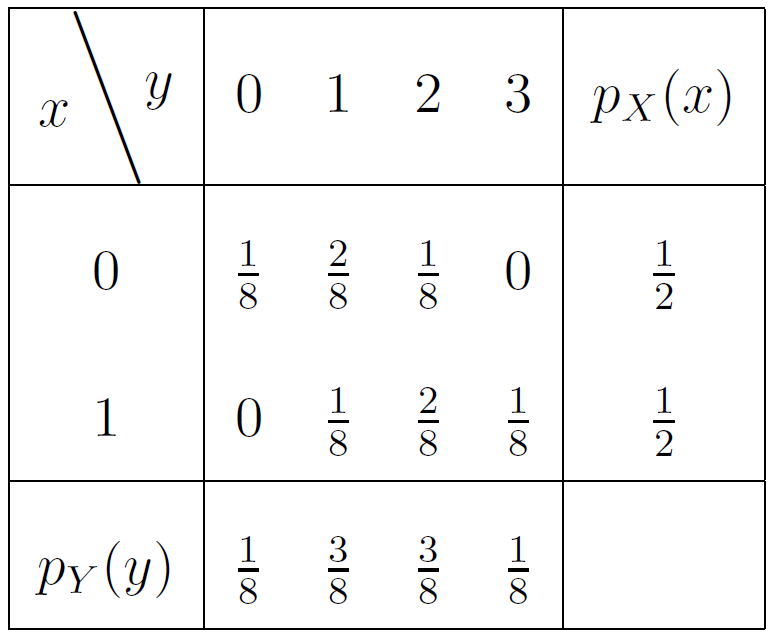
\includegraphics[scale=0.44]{randverteilung.png}
\end{center}
Aus den Randverteilungen kann man jedoch nicht ohne Weiteres die gemeinsame Verteilung herleiten, dazu fehlt Information über die \textit{Abhängigkeitsstruktur} der Zufallsvariable.

\begin{definition}[\textbf{Unabhängigkeit}]
Zufallsvariablen $X_1,\dots, X_n$ heissen \textit{unabhängig}, falls gilt
$$ F(x_1, \dots, x_n) = F_{X_1}(x_1) \cdots F_{X_n}(x_n)$$
\end{definition}
Folgendes Lemma gibt den Zusammenhang zu unabhängigen Ereignissen:
\begin{lemma}
Die diskreten Zufallsvariablen $X_1,\dots, X_n$ sind unabhängig\\ 
$\LLRA$ für beliebige Teilmengen $B_i \subseteq \mathcal{W}(X_i), i = 1\dots n$ sind die Ereignisse $A_i := \{X_i \in B_i\}$ für $i= 1\dots n$ unabhängig \\
$\LLRA$ für beliebige Teilmengen $B_i \subseteq \mathcal{W}(X_i), i = 1\dots n$ gilt:
$$ P[X_1 \in B_1, \dots, X_n \in B_n] = \prod_{i=1}^n P[X_i \in B_i]$$
\end{lemma}

\begin{satz}[\textbf{Funktionen auf Zufallsvariablen}]
Seien $X_1,\dots, X_n$ diskrete unabhängige Zufallsvariablen und $f_i :\R \to \R$ irgendwelche Funktionen. Sei weiter $Y_i := f_i(X_i)$ für $ 1 \leq 1 \leq n$. Dann sind die Zufallsvariablen $Y_1,\dots, Y_n$ ebenfalls unabhängig.
\end{satz}

\subsection{Funktionen von mehreren Zufallsvariablen}
Sind $X_1,\dots,X_n$ diskrete Zufallsvariablen, dann ist $Y = g(X_1,\dots,X_n)$ wieder eine Zufallsvariable für eine Funktion $g:\R^n \to \R$.

\begin{satz}
Seien $X_1,\dots,X_n$ diskrete Zufallsvariablen mit endlichen Erwartungswerten. Sei $Y = a + \sum_{i=0}^n  b_i X_i$ für Konstanten $a,b_i$. Dann gilt:
$$ \E[Y] = a + \sum_{i = 0}^n b_i \E[X_i]$$
\end{satz}

\begin{definition}[\textbf{Kovarianz}]
Seien $X,Y$ Zufallsvariablen auf einem Wahrscheinlichkeitsraum $(\Omega, \mathcal{F}, P)$ mit endlichen Erwartungswerten. Dann ist die \textit{Kovarianz} definiert als
$$ Cov(X,Y) := \E[(X-\E[X])(Y-\E[Y])] = \E[XY] - \E[X]\E[Y]$$
\end{definition}

\begin{definition}[\textbf{Korrelation}]
Die Korrelation von $X$ und $Y$ ist definiert durch
$$ \rho(X,Y) := \begin{cases} \frac{Cov(X,Y)}{\sigma(X)\sigma(Y)} & \mbox{falls } \sigma(X)\sigma(Y) > 0 \\ 0 & \mbox{sonst} \end{cases}$$
\end{definition}

\begin{satz}[\textbf{Wertebereich der Korrelation}]
Seien $X,Y$ wie in der Definition der Kovarianz, dann folgt aus der Cauchy-Schwarz Ungleichung, dass $|Cov(X,Y)| \leq \sigma(X)\sigma(Y)$, und damit folgt für die Korrelation
$$ -1 \leq \rho(X,Y) \leq 1$$
\end{satz}

Wir haben bereits gesehen, dass der Erwartungswert linear ist. Für die Varianz ist dies nicht ganz so einfach. Es gilt:

\begin{korollar}[\textbf{Summenformel für Varianzen}]
$$ \mbox{Var}\left[\sum_{i=1}^n X_i \right] = \sum_{i=1}^n \mbox{Var}[X_i] + 2 \cdot \sum_{i < j} Cov(X_i, X_j)$$
\end{korollar}
Ist $Cov(X,Y) = 0$, so nennt man $X$ und $Y$ \textbf{unkorreliert}. $\implies$ Linearität der Varianz gilt nur für unkorrelierte Zufallsvariablen. Für Produkte von Zufallsvariablen gilt:

\begin{satz}[\textbf{Produkte von Zufallsvariablen}]
Seien $X_1,\dots, X_n$  diskrete Zufallsvariablen mit endlichen Erwartungswerten. Falls $X_1,\dots,X_n$ unabhängig sind, dann gilt
$$\E\left[\prod_{i=1}^n X_i\right] = \prod_{i=1}^n \E[X_i]$$ Insbesondere sind $X_1,\dots,X_n$ paarweise unkorreliert und und daher gilt
$$ \mbox{Var}\left[\sum_{i=1}^n X_i\right] = \sum_{i=1}^n \mbox{Var}[X_i]$$ sofern die Varianzen existieren und endlich sind.
\end{satz}
\underline{Bemerkung:} Es gilt die Implikationskette: unabhängig $\implies$ paarweise unabhängig $\implies$ unkorreliert\\

\underline{Bemerkung:} Es gibt keine allgemeine Produktregel für Varianzen!

\subsubsection*{Faltung}
Seien $X,Y$ diskrete Zufallsvariablen mit gemeinsamer Gewichtsfunktion $p(x,y)$. Dann ist auch ihre Summe $Z:=X+Y$ diskret. Damit können wir die Gewichtsfunktion von $Z$ beschreiben durch
$$ p_Z(z) = P[Z=z] = \sum_{x_k \in \mathcal{W}(X)} P[X=x_k, Y = z-x_k] = \sum_{x_k \in \mathcal{W}(X)} p(x_k, z-x_k)$$ oder analog via Symmetrie $= \sum_{y_j\in\mathcal{W}(Y)} p(z-y_j, y_j)$. Dies ist ein völlig allgemeines Resultat. Sind nun $X$ und $Y$ unabhängig, dann gilt bekanntlich $p(x,y)= p_X(x) \cdot p_Y(y)$. Damit folgt die bekannte \textit{Faltung} der Gewichtsfunktionen $p_X$ und $p_Y$:
$$ p_Z(z) = \sum_{x_k \in \mathcal{W}(X)} p_X(x_k) \cdot p_Y(z-x_k) = \sum_{y_j \in \mathcal{W}(Y)} p_X(z-y_j) \cdot p_Y(y_j)$$ und schreiben dies kurz als $p_Z = p_X * p_Y = p_Y * p_X$.

\subsection{Bedingte Verteilungen}
Hier haben wir die gemeinsame Verteilung zweier Zufallsvariablen und wollen Informationen, die wir über eine der beiden Zufallsvariablen haben, ausnutzen um eine genauere Aussage über die andere Zufallsvariable zu machen.

\begin{definition}[\textbf{bedingte Gewichtsfunktion}]
$X,Y$ diskrete ZV mit gemeinsamer Gewichtsfunktion $p(x,y)$. Die \textit{bedingte Gewichtsfunktion} von $X$, gegeben dass $Y=y$, ist definiert als
$$ p_{X \with Y} (x \with y) := P[X=x \with Y=y] = \frac{P[X=x, Y = y]}{P[Y=y]} = \frac{p(x,y)}{p_Y(y)} $$
für $p_Y(y) >0$ und 0 sonst.
\end{definition}

\begin{lemma}[\textbf{Kriterium für Unabhängigkeit}]
Aus der Charakterisierung der Unabhängigkeit folgt sofort: \\
$X$ und $Y$ sind unabhängig $\LLRA$ für alle $y$ mit $p_Y(y)>0$ gilt: $p_{X \with Y} (x \with y) = p_X(x) \quad \forall x\in \mathcal{W}(X)$.
\end{lemma}
Eine symmetrische Aussage gilt natürlich, wenn $X$ und $Y$ vertauscht werden.\\

\underline{Bemerkung:} Man kann auch auf ein Ereignis bedingen, welches man dann mithilfe einer Indikatorvariable in eine Zufallsvariable verwandelt (siehe Beispiel Seite 64)

\section{Wichtige Diskrete Verteilungen}

\subsection{Diskrete Gleichverteilung}
Die \textit{diskrete Gleichverteilung} existiert nur auf einer endlichen Menge. Sie gehört zu einer ZV $X$ mit Wertebereich $\mathcal{W}$ und Gewichtsfunktion 
$$p_X(x_k) = P[X=x_k]=\frac{1}{N} \mbox{   für } k=1,\dots, N$$

\subsection{Unabhängige 0-1 Experimente}
Wir betrachten eine Folge gleichartiger Experimente, die alle nur mit Erfolg oder Misserfolg enden können und betrachten die Ereignisse $A_i = \{\mbox{Erfolg beim }i\mbox{-ten Experiment}\}$. Wir nehmen an, dass alle $A_i$ unabhängig sind und dass $P[A_i]=p$ für alle $i$. Wir können nun eine Indikatorfunktion $Y_i = I_{A_i}$ für jedes $i$ definieren, und danach die Folge von Ereignissen als Folge von 0 und 1 codieren. Dies werden wir für die nächsten Verteilungen brauchen.

\subsection{Bernoulli-Verteilung}
Wir machen ein einziges 0-1 Experiment und nennen das Ergebnis $X \implies X \sim Be(p)$ 
\begin{itemize}
\item \textbf{Wertebereich:} $\mathcal{W}(X) = \{0,1\}$
\item \textbf{Gewichtsfunktion:} $p_X(x) := \begin{cases} P[X=1]=p & \mbox{falls } x=1 \\ P[X=0]=1-p & \mbox{falls } x=0 \end{cases}\quad \quad \quad$ also insgesamt $p_X(x)= p^x(1-p)^{1-x}$
\item \textbf{Erwartungswert:} $\E[X]=p \quad \quad \quad$
\item \textbf{Varianz:} $\mbox{Var}[X] = p(1-p)$
\end{itemize}

\subsection{Binomialverteilung}
Beschreibt die Anzahl der Erfolge bei $n$ unabhängigen 0-1 Experimenten mit Erfolgsparameter $p$. Sei $X$ die Anzahl der Erfolge $\implies X \sim Bin(n,p)$.
\begin{itemize}
\item \textbf{Wertebereich:} $\mathcal{W}(X) = \{0,1,2,\dots,n\}$
\item \textbf{Gewichtsfunktion:} $p_X(k) = P[X=k] = \binom{n}{k} p^k (1-p)^{n-k} \quad \quad \mbox{für } k = 0,1,\dots, n$
\item Summe von $n$ unabhängigen bernoulli-verteilten ZV mit gleichem Parameter $p$
\item \textbf{Erwartungswert:} $\E[X] = \sum_{i=1}^n \E[Y_i] = np$
\item \textbf{Varianz:} Var$[X] = \sum_{i=1}^n \mbox{Var}[Y_i] = np(1-p)$
\end{itemize}
Für die Binomialverteilung existiert eine Rekursionsformel:
$$p(k+1, n) = \frac{p}{1-p} \frac{n-k}{k+1} p(k,n)$$

\subsection{Geometrische Verteilung}
Wir betrachten eine unendliche Folge von unabhängigen 0-1 Experimenten mit Erfolgsparameter $p$ und warten auf den ersten Erfolg. Sei $X = \inf \{i\in\N \with A_i$ tritt ein $\} = \inf \{i \in \N \with Y_i = 1\}$ die Wartezeit $\implies X \sim Geom(p)$.
\begin{itemize}
\item \textbf{Wertebereich:} $\mathcal{W}(X)=\{1,2,\dots\} = \N$
\item \textbf{Gewichtsfunktion:} $p_X(k) = P[X=k] = p(1-p)^{k-1} \quad \quad $ für $k=1,2,3\dots $
\item \textbf{Erwartungswert:} $P[X > l] = (1-p)^l \implies \E[X] = \sum_{l=0}^\infty P[X>l] = \sum_{l=0}^\infty (1-p)^l = \frac{1}{1-(1-p)} = \frac{1}{p}$
\item \textbf{Varianz:} Var$[X] = \frac{1-p}{p^2}$
\end{itemize}

\begin{mdframed}
\subsubsection*{Coupon Collector Problem}
\underline{Gesucht:} Anzahl Käufe, bis man alle Bilder/Coupons besitzt. $\to$ Sei $X_i$ die Anzahl Käufe bis zum $i$-ten verschiedenen Bild, unter Annahme dass man schon $i-1$ Bilder besitzt. $\implies X_i$ sind geometrisch verteilt, und $X= \sum_{i=1}^n$. Dann kann die Linearität des Erwartungswert ausgenutzt werden, um $\E[X]$ zu berechnen.
\end{mdframed}

\subsection{Negativbinomiale Verteilung}
Betrachten wir erneut eine unendliche Folge von unabhängigen 0-1 Experimenten mit Erfolgsparameter $p$. Nun interessiert uns allerdings die Wartezeit auf den $r$-ten Erfolg, wobei $r\in \N$. Dies ist eine Verallgemeinerung der \textit{geometrischen Verteilung}, welche den Spezialfall $r=1$ abdeckt. Die Zufallsvariable $X$ lässt sich schreiben als
$$ X = \inf \left\{k \in \N \: \middle| \: \sum_{i=1}^k I_{A_i} = r\right\} = \inf \left\{k \in \N \: \middle|\: \sum_{i=1}^k Y_i = r\right\}$$
Wir schreiben $X \sim NB(r,p)$
\begin{itemize}
\item \textbf{Wertebereich:} $\mathcal{W}(X) = \{r, r+1, r+2, \dots\}$
\item \textbf{Gewichtsfunktion:} $p_x(k) = P[X=k] = \binom{k-1}{r-1} p^r (1-p)^{k-r}$
\item Sind ZV $X_1,\dots,X_r \sim Geom(p)$ und unabhängig $\implies \sum_{i=1}^r X_i =: X \sim NB(r,p)$
\item \textbf{Erwartungswert:} $\E[X] = \sum_{i=1}^r \E[X_i] = \frac{r}{p}$
\item \textbf{Varianz:} Var$[X] = \sum_{i=1}^r \mbox{Var}[X_i] = \frac{r(1-p)}{p^2}$
\end{itemize}

\subsection{Hypergeometrische Verteilung}
Wir unterscheiden zwei Arten von Gegenständen. Gegeben sind $n$ Gegenstände, $r$ davon von Typ 1 und $n-r$ von Typ 2. Man zieht nun $m$ Gegenstände ohne Zurücklegen und interessiert sich für die Anzahl der Gegenstände von Typ 1. Sei $X$ diese Anzahl $\implies X \sim Hypergeometric(n,m,r)$.
\begin{itemize}
\item \textbf{Wertebereich:} $\mathcal{W}(X) = \{0,1, \dots, \min(m,r)\}$
\item \textbf{Gewichtsfunktion:} $p_X(k) = \frac{\binom{r}{k} \binom{n-r}{m-k}}{\binom{n}{m}}$ für $k\in \mathcal{W}(X)$.
\item \textbf{Erwartungswert:} $\E[X] = \frac{rm}{n}$
\item \textbf{Varianz:} Var$[X] = \frac{(n-r) n m (n-m)}{(2n-r)^2(n-1)}$
\end{itemize}
\underline{Bemerkung:} Die Varianz der hypergeometrischen Verteilung ist sehr schwierig herzuleiten, und wird im Skript genau wie der Erwartungswert gar nicht aufgeführt.

\subsection{Poisson-Verteilung}
Die Poisson-Verteilung erhält man nicht aus einem konkreten Experiment, sondern durch einen Grenzübergang aus der Binomialverteilung $\implies$ gut zur Modellierung von seltenen Ereignissen. Man schreibt $X \sim \mathcal{P}(\lambda)$ für ein $\lambda \in (0, \infty)$
\begin{itemize}
\item \textbf{Wertebereich:} $\mathcal{W}(X) = \{0,1,2,\dots\} = \N_0$
\item \textbf{Gewichtsfunktion:} $p_X(k) = e^{-\lambda} \frac{\lambda^k}{k!}$ für $k= 0,1,2,\dots$
\item \textbf{Erwartungswert:} $\E[X] = \lambda$
\item \textbf{Varianz:} Var$[X] = \lambda $
\end{itemize}

\begin{mdframed}
\subsubsection*{Herleitung}
Sei $X_n$ für jedes $n$ eine ZV mit $X \sim Bin(n,p)$ und $np_n = \lambda$ und damit $p_n = \frac{\lambda}{n}$, welches für $n\to\infty$ gegen 0 geht. Bekanntlich gilt
\begin{eqnarray}
P[X_n = k] & = & \binom{n}{k} p_n^k (1-p_n)^{n-k} \\ & = & \frac{n!}{k!(n-k)!} \left(\frac{\lambda}{n} \right)^k \left(1-\frac{\lambda}{n}\right)^{-k} \\
& = & \frac{\lambda^k}{k!} \cdot \underbrace{\frac{n(n-1) \cdots (n-k+1)}{n^k}}_{= 1 \mbox{ für } n\to \infty} \cdot \underbrace{\left(1-\frac{\lambda}{n} \right)^n}_{=e^{-\lambda} \mbox{ für } n \to \infty} \cdot \underbrace{\left(1-\frac{\lambda}{n}\right)^{-k}}_{=1 \mbox{ für } n \to \infty}
\end{eqnarray}
wobei die Klammern den Grenzwert für $n\to \infty$ und $k$ fixiert angeben. Damit sehen wir, folgendes Resultat:
$$ \lim_{n\to\infty} P[X_n = k] = e^{-\lambda} \frac{\lambda^k}{k!}=P[X=k]$$
Damit lässt sich die oft komplizierte Binomialverteilung relativ gut \textit{approximieren}, wenn $\lambda = np$. Man verwendet als Faustregel, dass die Approximation verwendet werden kann, wenn $np^2 \leq 0.05$
\end{mdframed}
\section{Allgemeine Zufallsvariablen}

\subsection{Grundbegriffe}
\begin{definition}[\textbf{Zufallsvariable}]
Sein $(\Omega,\mathcal{F}, P)$ ein Wahrscheinlichkeitsraum. Eine \textit{Zufallsvariable} (ZV) auf $\Omega$ ist eine messbare Funktion $X:\Omega \to \R$, das bedeutet, dass die Menge $\{X \leq t\} = \{ \omega \with X(\omega) \leq t\}$ für jedes $t$ ein beobachtbares Ereignis, also $\in \mathcal{F}$ sein muss. \\
Die \textit{Verteilungsfunktion} (VF) von $X$ ist die Abbildung $F_X:\R\to [0,1]$ mit
$$ t \mapsto F_X(t) := P[X \leq t] := P[\{ \omega \with X(\omega) \leq t\}]$$
\end{definition}
Wir betrachten nur messbare Zufallsvariablen in dieser Vorlesung.

\begin{satz}[\textbf{Eigenschaften der Verteilungsfunktion}]
$F_X$ hat folgende Eigenschaften:
\begin{itemize}
\item[(i)] $F_X$ ist \textit{wachsend} und \textit{rechtsstetig}: $F_X(s) \leq F_X(t)$ für $s\leq t$ und $F_X(u) \to F_X(t)$ für $u\to t$ mit $u>t$.
\item[(ii)] $lim_{t\to -\infty} F_X(t) = 0$ und $\lim_{t\to\infty} F_X(t) =1 $
\end{itemize}
\end{satz}

Das stochastische Verhalten einer ZV $X$ wird durch die \textit{Verteilung} beschrieben, d.h. das Wahrscheinlichkeitsmass $\mu_X$, welches durch $\mu_X(B) = P[X\in B]$ definiert ist. Sobald die Verteilungsfunktion $F_X$ bekannt ist, ist das Mass $\mu_X$ festgelegt, nämlich durch den Zusammenhang
$$F_X(t) = \mu_X\left((-\infty, t]\right)$$
Anstelle der Gewichtsfunktion aus dem diskreten Fall verwenden wir die \textit{Dichtefunktion}, sofern diese existiert.

\begin{definition}[\textbf{Dichtefunktion}]
Eine ZV $X$ mit Verteilungsfunktion $F_X(t) = P[X \leq t]$ heisst \textit{(absolut) stetig} mit Dichtefunktion $f_X:\R\to [0,\infty)$, falls gilt
$$ F_X(t) = \int \limits_{-\infty}^t f_X(s) \: ds \quad \quad \mbox{ für alle } t \in \R. $$
\end{definition}
\underline{Bemerkung:} $X$ heisst stetig, falls $F_X$ nur stetig ist. Eine ZV $X$ mit einer Dichte hat aber eine VF $F_X$, die fast überall differenzierbar ist. Dafür verwenden wir den Begriff \textit{\textcolor{blue}{stetig mit Dichte}}.

\begin{satz}[\textbf{Eigenschaften der Dichte}]
Die Dichtefunktion $f_X$ hat folgende Eigenschaften:
\begin{itemize}
\item[(i)] $f_X \geq 0$ und $f_X = 0$ ausserhalb des Wertebereichs $\mathcal{W}(X)$
\item[(ii)] $ \int \limits_{-\infty}^{\infty} f_X(s) \: ds = 1$ (dies folgt aus Eigenschaft (ii), 2. GW von der Verteilungsfunktion.)
\end{itemize}
In beinahe allen praktischen Beispielen ist $f_X$ zusätzlich stetig oder zumindest stückweise stetig.
\end{satz}

Die Dichtefunktion ist beinahe analog zur Gewichtsfunktion für diskrete Zufallsvariablen, jedoch unterscheidet sie sich in Punktwahrscheinlichkeiten. Es gilt
\begin{align*}
P[a < X \leq b] &= P[X \leq b] - P[X \leq a] = F_X(b) - F_X(a) = \int \limits_a^b f_X(s) \: ds \\&\implies P[X\in B] = \int\limits_B f_X(s)\: ds
\end{align*}
und betrachtet man nun einen Grenzwert, so erhält man
$$ \lim_{\epsilon \to 0^+} P[t-\epsilon < X \leq t + \epsilon] = \lim_{\epsilon \to 0^+} \int \limits_{t-\epsilon}^{t+\epsilon} f_X(s) \: ds = 0 = P[X=t]$$
Damit ist die Punktwahrscheinlichkeit an jedem Punkt = 0. Jedoch gilt für kleine $\epsilon$ (wir verwenden hier $\epsilon= dt$) das Folgende:
$$ P\left[X\in (t,t+dt]\right] = f_X(t) dt$$
In allen vernünftigen Situationen gilt also der folgende Zusammenhang zwischen Dichtefunktion und Verteilung:
\begin{center}
Dichtefunktion = Ableitung der Verteilungsfunktion
\end{center}
Vom diskreten zum stetigen Fall kommt man , indem Summen durch Integrale und die Gewichtsfunktion durch die Dichte ersetzt.

\subsection{Normalverteilung}
Normalverteilung oder \textit{Gauss-Verteilung} nimmt zwei Parameter $\mu \in \R,\: \sigma^2 > 0$. Ihre Dichte ist symmetrisch um $\mu$ und hat eine glockenförmige Gestalt.
\begin{itemize}
\item \textbf{Wertebereich:} $\mathcal{W}(X) = \R$
\item \textbf{Dichtefunktion:} $f_X(t) = \frac{1}{\sigma \sqrt{2\pi}}e^{- \frac{(t-\mu)^2}{2\sigma^2}}$ für $t\in \R$
\item \textbf{Erwartungswert:} $\E[X] = \mu$ und \textbf{Varianz:} Var$[X] = \sigma^2$
\item \textbf{Verteilungsfunktion:} entspricht dem Integral von der Dichtefunktion über dem Intervall $[-\infty, t)$, es existiert jedoch kein geschlossener Term.
\item \textbf{Notation:} $X \sim \mathcal{N}(\mu, \sigma^2)$
\end{itemize}
\begin{center}
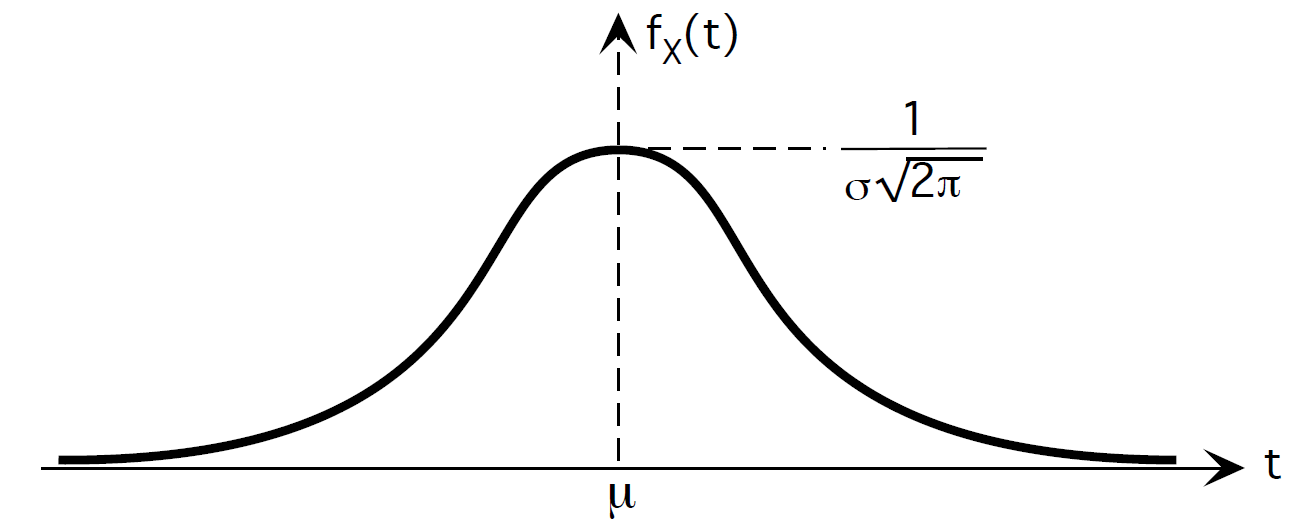
\includegraphics[scale=0.3]{normalverteilung.png}
\end{center}
Mit einer Normalverteilung können z.b: die Streuung von Messwerten um ihren Mittelwert, Gewichte bzw. Grössen in Bevölkerungen, Leistungen in IQ-Tests und viele mehr modelliert werden. Der Grund für die Wichtigkeit der Normalverteilung liegt im \textit{Zentralen Grenzwertsatz}, der in Kapitel 5 besprochen wird.

\subsubsection{Standard-Normalverteilung}
Die \textit{Standard-Normalverteilung} gibt die beiden Parameter vor: $\mu = 0$ und $\sigma^2 = 1$.
\begin{itemize}
\item \textbf{Dichtefunktion:} $\phi(t) = \frac{1}{\sqrt{2\pi}}e^{-\frac{t^2}{2}}$
\item \textbf{Verteilungsfunktion:} Wieder existiert kein geschlossener Ausdruck, jedoch ist das Integral \textit{tabelliert}:
$$ \Phi(t) = \int\limits_{-\infty}^t \phi(s) \: ds = \frac{1}{\sqrt{2\pi}} \int\limits_{-\infty}^t e^{-\frac{s^2}{2}}\: ds$$
\end{itemize}
\underline{Wichtig:} $X \sim \mathcal{N}(\mu, \sigma^2) \implies  \frac{X-\mu}{\sigma} \sim \mathcal{N}(0,1)$. Daraus folgt unmittelbar, dass es ausreicht, nur die Werte von $\Phi(t)$ zu tabellieren, denn es gilt:
$$ F_X(t) = P[X \leq t] = P\left[ \frac{X-\mu}{\sigma} \leq \frac{t-\mu}{\sigma} \right] = \Phi\left(\frac{t-\mu}{\sigma}\right)$$


\subsection{Erwartungswerte}
Eine beliebige reellwertige ZV $X$ kann immer durch eine Folge diskreter ZV approximiert werden. Ist bspw. $X \geq 0$, dann kann man 
$$ X_N := \sum_{k=1}^{n2^n} \frac{k-1}{2^n}I_{\{\frac{k-1}{2^n} \leq X \leq \frac{k}{2^n}\}} + nI_{\{X \geq n\}}$$
für $X_n \nearrow X$ wählen und erhält den Erwartungswert als $$ \E[X] := \lim_{n\to\infty} \E[X_n]$$
Für allgemeine Zufallsvariablen zerlegt man $X = X^+ - X^- := \max{(X,0)} - \max{(-X,0)}$ mit $X^+, X^- \geq 0$ und setzt dann $\E[X] = \E[X^+] - \E[X^-]$. Sind diese beiden Erwartungswerte nicht endlich, so existiert der Erwartungswert von $X$ nicht (in $\R$).\\

\underline{\textbf{Erwartungswert berechnen:}} Ist $X$ stetigt mit einer Dichte $f_X(x)$, so gilt (sofern konvergent):
$$ \E[X] = \int \limits_{-\infty}^{\infty} x \cdot f_X(x) \: dx$$
\underline{\textit{Cauchy-Verteilung:}} $\mathcal{W}(X) = \R$ mit Dichte $f_X(x) = \frac{1}{\pi}\frac{1}{1+x^2}$ und Verteilung $F_X(x) = \frac{1}{2} + \frac{1}{\pi} \arctan(x)$. Es gilt, dass für zwei unabhängige, $\mathcal{N}(0,1)$-verteilte ZV $X,Y$ ihr Quotient $Z := X/Y$ gerade \textit{Cauchy-verteilt} ist. Die Charakteristik liegt darin, dass die Dichte für $|x| \to \infty$ sehr langsam gegen 0 geht, d.h. auch sehr grosse Werte nocht mit substantieller Wahrscheinlichkeit angenommen werden. Ein Erwartungswert existiert nicht.\\

\begin{satz}
Seien $X$ und $Y=g(X)$ zwei ZV. Ist $X$ stetig mit Dichte $f_X(x)$ dann gilt (sofern das Integral konvergiert)
$$ \E[Y] = \E[g(X)] = \int \limits_{-\infty}^{\infty} g(x) \cdot f_X(x) \: dx$$
\end{satz}
Weitere Eigenschaften für Erwartungswerte gelten analog zum diskreten Fall, einzig die konkreten Berechnungen unterscheiden sich.

\subsection{Momente \& Absolute Momente}

\begin{definition}[\textbf{Moment}]
Sei $X$ eine Zufallsvariable und $p\in R_+$. Wir definieren:
\begin{itemize}
\item \textit{das} $p$\textit{-te absolute Moment von} $X$ durch $M_o := \E[|X|^p ]$ (kann $\infty$ sein)
\item falls $M_n < \infty$ für ein $n$, dann ist das $n$\textit{-te (rohe) Moment von} $X$ durch $m_n:= \E[X^n]$ definiert.
\item Das $n$\textit{-te zentralisierte Moment von} $X$ durch $m_n:= \E[(X - \E[X])^n]$ definiert.
\end{itemize}
\end{definition}
Damit folgt sofort:
\begin{korollar}
$M_n < \infty$ für $n\in\N \implies |m_n| \leq M_n$
\end{korollar}
Hat $X$ eine Dichte $f_X$, dann gilt zudem für das absolute Moment
$$ M_p = \int \limits_{-\infty}^\infty |x|^p f_X(x) \ dx$$ 
Gilt dann $M_n < \infty$ für ein $n\in\N$, dann können wir auch das $n$-te Moment per Integral bestimmen:
$$ m_n = \int \limits_{-\infty}^{\infty} x^n f_X(x) \ dx $$

\begin{satz}
Sei $X$ ZV und $p,q \in R_+$. Dann:
$$ p \leq q \; \land \; M_q < \infty \implies M_p < \infty$$
\end{satz}
\subsection{Gemeinsame Verteilungen, Unabhängige Zufallsvariablen}

\begin{definition}[\textbf{Gemeinsame Verteilung}]
Die \textit{gemeinsame Verteilungsfunktion} von $n$ ZV $X_1,\dots, X_n$ ist die Abbildung $F:\R^n \to [0,1]$ mit:
$$ (x_1,\dots, x_n) \mapsto F(x_1, \dots, x_n) := P[X_1 \leq x_1, \dots, X_n \leq x_n]$$
Lässt sich $F$ für eine Funktion $f:\R^n \to [0, \infty)$ schreiben als 
$$ F(x_1,\dots, x_n) = \int\limits_{-\infty}^{x_1} \dots \int \limits_{-\infty}^{x_n} f(t_1, \dots, t_n) dt_n \dots dt_1 $$
dann heisst $f(x_1,\dots, x_n)$ die \textit{gemeinsame Dichte} von $X_1, \dots, X_n$.
\end{definition}

\begin{korollar}[\textbf{Eigenschaften der Dichte}]
Für die gemeinsame Dichte von $X_1,\dots,X_n$ gilt:
\begin{itemize}
\item[(i)] $f(x_1,\dots, x_n) \geq 0$ und $=0$ ausserhalb $\mathcal{W}(X_1, \dots, X_n)$
\item[(ii)] $ \iiint \limits_{\R^n} f(x_1, \dots, x_n) dx_n \dots dx_1 = 1$
\item[(iii)] $P[(X_1,\dots, X_n) \in A] = \iiint \limits_{(x_1,\dots,x_n) \in A} f(x_1, \dots, x_n) dx_n \dots dx_1$ für $A\subseteq \R^n$.
\end{itemize}
\end{korollar}

\begin{definition}[\textbf{Randverteilung}]
Haben $X,Y$ die gemeinsame Verteilungsfunktion $F$, dann sind $F_X:\R\to[0,1]$ und $F_Y:\R\to[0,1]$ die Verteilungsfunktionen der \textit{Randverteilung} von $X$ bzw. $Y$ und sind definiert als:
$$ x \mapsto F_X(x) := P[X \leq x] = P[X \leq x, Y < \infty] = \lim_{y\to \infty} F(x,y)$$
$$ y \mapsto F_Y(y) := P[Y \leq y] = P[X < \infty, Y \leq y] = \lim_{x\to \infty} F(x,y)$$
Haben $X,Y$ eine gemeinsame Dichte $f$, dann haben auch die Randverteilungen Dichten $f_X:\R\to [0, \infty)$ und $f_Y:\R \to [0, \infty)$ mit
$$ f_X(x) = \int\limits_{-\infty}^{\infty} f(x,y) dy \quad \quad \quad \quad \quad f_Y(y) = \int \limits_{-\infty}^{\infty} f(x,y) dx$$
\end{definition}

\begin{definition}[\textbf{Unabhängigkeit}]
Die ZV $X_1,\dots,X_n$ heissen \textit{unabhängig} $LLRA$ $F(x_1,\dots,x_n) = F_{X_1}(x_1) \cdots F_{X_n}(x_n)$.\\
Hat man stetige Zufallsvariablen mit Dichten, dann ist die gemeinsame Dichtefunktion das Produkt der Randdichten, also
$$ f(x_1, \dots, x_n) = f_{X_1}(x_1) \cdots f_{X_n}(x_n)$$
\end{definition}

\subsection{Bedingte Verteilungen usw}

\begin{definition}[\textbf{Bedingte Dichte, Verteilungsfunktion und Erwartungswert}]

$$ f_{X_1 \mid X_2}(x_1\mid x_2) = \frac{f_{X_1, X_2}(x_1, x_2)}{f_{X_2}(x_2)}$$
$$ P(Y > t\mid Y < a) = \frac{P[t < Y < a]}{P[Y < a]}$$

$$ E[X_1 \mid X_2](x_2) = \int x_1 f_{X_1 \mid X_2}(x_1\mid x_2)\ dx_1$$
Mit Trick:
\begin{align*}
	E[X_1] = E[E[X_1 \mid X_2]] &= \int E[X_1 \mid X_2](x_2) f_{X_2}(x_2) dx_2\\
	&=\int \int x_1 f_{X_1, X_2}(x_1, x_2) dx_1 dx_2
\end{align*}
Anm. $E[X_1 \mid X_2](x_2) = E[X_1 \mid X_2=x_2]$ 
\end{definition}

\subsection{Funktionen und Transformationen von Zufallsvariablen}
\subsubsection*{Summen}
Für $Z=X+Y$ suchen wir die Verteilungsfunktion $F_Z(z) = P[Z \leq z] = P[X+Y \leq z]$. Dies kann man als Punktemenge im $\R^2$ auffassen, nämlich $A_z := \{(x,y) \in \R^2 \with x+y \leq z\}$. Damit ist $F_Z(z) = P[(X,Y) \in A_z]$. Damit erhält man 
$$F_Z(z) = \int \limits_{-\infty}^\infty \int \limits_{-\infty}^{z-x} f(x,y) \ dy \ dx $$
Substituiere nun $v=x+y \Rightarrow y = v-x, dy = dv$ so erhält man
\begin{align*}
	F_Z(z) &= \int \limits_{-\infty}^\infty \int \limits_{-\infty}^z f(x,v-x) \ dv \ dx = \int \limits_{-\infty}^z \int \limits_{-\infty}^\infty f(x,v-x) \ dx \ dv \\&\implies f_Z(z) = \frac{d}{dz}F_Z(z) = \int \limits_{-\infty}^\infty f(x,z-x) \ dx = \int \limits_{-\infty}^\infty f(z-y,y) \ dy
\end{align*}
womit wir also auch die Dichte erhalten haben. Das letzte Gleichheitszeichen gilt wegen Symmetrie zwischen $X,Y$. Sind $X,Y$ unabhängig, so gilt $f(x,y) = f_X(x)\cdot f_Y(y)$ und dann ist $f_Z$ die \textit{Faltung} von $f_X$ und $f_Y$.

\subsubsection*{Transformationen}
Sei $X$ ZV mit Verteilung und Dichte. Sei $g:\R\to\R$ messbare Funktion. Betrachte $Y = g(X)$, wir suchen Verteilung und Dichte (falls existent) von $Y$. Allgemein löst man dieses Problem wie folgt:
$$ F_Y(t) = P[Y \leq t] = P [g(X) \leq t] = \int \limits_{A_g} f_X(s) \ ds $$ mit $A_g := \{ s\in \R \with g(s) \leq t\}$. Die Dichtefunktion (falls existent) erhält man dann durch Ableiten der Verteilung.
\subsubsection*{Awendung der Transformation}
\begin{satz}
Sei $F$ stetige, streng-monoton wachsende Verteilungsfunktion mit Umkehrfunktion $F^{-1}$. Dann:
$$ X \sim \mathcal{U}(0,1) \quad \land \quad Y = F^{-1}(X) \implies Y \mbox{ hat Verteilungsfunktion } F.$$
\end{satz}
Dieser Satz erlaubt die Konstruktion einer Zufallsvariablen $Y$ mit einer gewünschten Verteilungsfunktion $F$, wenn man eine Zufallsvariable $X \sim \mathcal{U}(0,1)$ zur Hand hat. Damit kann man beispielsweise eine Verteilung mit einem Computer simulieren. Ein Zufallszahlengenerator produziert in einem gewissen Sinn eine Folge von $\mathcal{U}(0,1)$-verteilten Zufallsvariablen. $\implies$ $F^{-1}($Zufallszahlengenerator$)$ simuliert also die Verteilung $F$.
\section{Ungleichungen und Grenzwertsätze}
\subsection{Wahrscheinlichkeit \& Konvergenz}
\begin{definition}[\textbf{Konvergenz in Wahrscheinlichkeit}]
Sei $X_1,X_2,\dots$ und $Y$ ZV auf gemeinsamen Wahrscheinlichkeitsraum.
\begin{itemize}
\item[(i)] $X_1,X_2,\dots$ konvergiert gegen $Y$ \textit{in Wahrscheinlichkeit} falls $$\forall \varepsilon >0. \quad \lim_{n\to \infty} P[ |X_n -Y| > \varepsilon] = 0$$
\item[(ii)] Für $p>0$ konvergiert die Folge $X_1,X_2,\dots$ gegen $Y$ \textit{in} $L^p$ falls $$\lim_{n\to\infty} \E[ |X_n - Y|^p] = 0$$
\item[(iii)] $X_1,X_2,\dots$ konvergiert gegen $Y$ \textit{P-fast sicher} falls $$ P\left[ \lim_{n\to\infty} X_n = Y \right] = P \left[ \left \{ \omega \in \Omega \with \lim_{n\to\infty} X_n(\omega) = Y(\omega) \right \} \right] = 1$$
\end{itemize}
\end{definition}

\begin{definition}[\textbf{Konvergenz in Verteilung}]
Seien $X_1,X_2,\dots,$ und $Y$ ZV auf möglicherweise verschiedenen Wahrscheinlichkeitsräumen mit Verteilungsfunktionen $F_1,F_2,\dots$ und $F_Y$. Dann konvergiert $X_1,X_2, \dots$ gegen $Y$ \textit{in Verteilung} falls
$$ \lim_{n\to\infty} F_n(x) = F_Y(x) \quad \quad \mbox{für alle } x\in R, \mbox{wo } F_Y \mbox{ stetig ist}$$
\end{definition}

\begin{satz}
Es gilt folgende Äquivalenz:
$$ X_1,X_2,\dots \mbox{ konvergiert in Verteilung gegen } Y \LLRA \lim_{n\to\infty} \E[f(X_n)] = \E[f(Y)] \mbox{ für jedes beschränkte stetige } f:\R\to\R$$
\end{satz}
\subsection{Ungleichungen}
\begin{satz}[\textbf{Markov-Ungleichung}]
Sei $X$ eine Zufallsvariable und $g:\mathcal{W}(X)\to [0, \infty)$ eine wachsende Funktion. Für jedes $c \in \R$ mit $g(c) > 0$ gilt dann:
$$ P[X \geq c] \leq \frac{\E[g(X)]}{g(c)}$$
\end{satz}
\underline{Bemerkung:} Insbesondere gilt der satz für die Identitätsfunktion $g=id$. Daraus folgt unmittelbar:
\begin{satz}[\textbf{Chebyshev-Ungleichung}]
Sei $Y$ Zufallsvariable mit endlicher Varianz. Für jedes $b>0$ gilt dann:
$$ P\left[ |Y-\E[Y]| \geq b \right] \leq \frac{\mathrm{Var}[Y]}{b^2}$$
\end{satz}
\begin{proof}
Wähle $X:=|Y-\E[Y]|$ und $g(x) =x^2 $ für $x\geq 0 \implies \E[g(Y)] = \mathrm{Var}[Y]$.
\end{proof}

\subsection{Gesetz der grossen Zahlen}
Wir betrachten nun Folgen von Zufallsvariablen mit dem gleichen Erwartungswert und der gleichen Varianz. Uns interessiert das Verhalten des arithmetischen Mittel dieser Folge von Zufallsvariablen.
\begin{satz}[\textbf{Schwaches Gesetz der grossen Zahlen}]
Sei $X_1, X_2, \dots$ eine Folge von unabhängigen ZV mit $\E[X_i]= \mu $ und Varianz $\mathrm{Var}[X_i] = \sigma^2$. Sei $\overline{X_n} =\frac{1}{n}\sum_{i=1}^n X_i$. Dann konvergiert $\overline{X_n}$ für $n\to \infty$ in Wahrscheinlichkeit/stochastisch gegen $\mu$.
\end{satz}
\begin{proof}
Betrachte Linearität des EW: $\E[\overline{X_n}] = \frac{1}{n}\sum_{i=1}^n \E[X_i] = \mu$. Da die ZV paarweise unkorreliert sind, gilt auch die Linearität der Varianz und somit $\mathrm{Var}[\overline{X_n}] = \frac{1}{n}\sum_{i=1}^n \mathrm{Var}[X_i] = \frac{\sigma^2}{n}$. Die Chebyshev-Ungleichung liefert damit:
$$ P \left[ |\overline{X_n}-\mu|> \varepsilon \right] \leq \frac{\mathrm{Var}[\overline{X_n}}{\varepsilon^2} = \frac{\sigma^2}{n\cdot \varepsilon^2}$$
Dieser Term geht für jedes beliebige $\varepsilon>0$ gegen 0, was \textit{Def. 5.1 (i)} entspricht.
\end{proof}
\underline{Bemerkung 1:} Es genügt bereits, wenn $X_i$ nur paarweise unkorreliert sind.\\
\underline{Bemerkung 2:} Die Existenz des Erwartungswerts ist essentiell, damit das Gesetz gilt: So existiert bspw kein Erwartungswert für die bereits eingeführte \textit{Cauchy-Verteilung}. Damit konvergiert $n\mapsto \overline{X_n}(\omega)$ nicht, denn Summen von Cauchy-verteilten Zufallsvariablen sind wiederum Cauchy-verteilt.

\subsubsection*{Monte-Carlo-Integration}
Wir wollen für $h:[0,1]^d \to \R$ ein Integral $I:= \int_{[0,1]^d} h(\vec{x}) \ d\vec{x}$ berechnen, welches auch numerisch schwer lösbar ist. Dafür können wir $I$ als einen Erwartungswert auffassen. Sei $d=1$. Ist $U \sim \mathcal{U}(0,1)$, dann gilt 
$$ \E[h(U)] ) = \int_{\R} h(x)f_U(x) \ dx = \int_0^1 h(x) \ dx = I$$
Die letzte Gleichheit gilt, weil die Dichte von $U$ auf $[0,1]$ konstant 1 ist, und sonst 0. Deshalb können wir mit einem Zufallszahlengenerator eine Folge $U_1,U_2,\dots$ generieren mit $U_i \sim \mathcal{U}(0,1)$ und den Wert von $I$ mit dem schwachen GGZ approximieren:
$$ \overline{h(U_n)} = \frac{1}{n} \sum_{i=1}^n h(U_i)$$ 
Damit ist aber auch gleich klar, wieso man eine stärkere Aussage möchte, denn der berechnete Wert liegt nur mit grosser Wahrscheinlichkeit sehr nahe bei $I$, aber man weiss nicht, ob eine feste Realisierung $\omega$ in dieser guten Approximationsmenge liegt.

\begin{satz}[\textbf{Starkes Gesetz der grossen Zahlen}]
Sei $X_1,X_2,\dots$ eine Folge von unabhängigen Zufallsvariablen mit gleicher Verteilung und EW $\mu$ endlich. Für das arithmetische Mittel $\overline{X_n} := \frac{1}{n} \sum_{i=1}^n X_i$ gilt dann, dass $\overline{X_n}$ \textit{P-fast sicher} (P.f.s.) gegen $\mu$ konvergiert, also
$$ P \left[ \left \{ \omega \in \Omega \with \overline{X_n}(\omega) \underset{n\to\infty}{\longrightarrow} \mu \right \} \right] $$
\end{satz}
Für die Monte-Carlo Integration bedeutet dies, dass unserer berechneter Wert mit Wahrscheinlichkeit 1 nahe bei $I$ liegt. Schlechte Approximationen sind zwar möglich, aber mit Wahrscheinlichkeit 0.

\subsection{Zentraler Grenzwertsatz}
Wir bezeichnen unabhängige gleichverteilte Zufallsvariablen als \textit{i.i.d.} für \textit{independent identically distributed}.
\begin{satz}[\textbf{Zentraler Grenzwert}]
Sei $X_1,X_2,\dots$ eine Folge von i.i.d. ZV mit EW $\mu$ und Varianz $\sigma^2$. Für die Summe $S_n = \sum_{i=1}^n X_i$ gilt dann:
$$ \lim_{n\to\infty} P\left[\frac{S_n - n\mu}{\sigma \sqrt{n}} \leq x \right] = \Phi(x) \quad \quad \forall x\in\R$$
Für praktische Anwendungen existieren zwei alternative Notationen:
\begin{itemize}
\item $P[S_n^* \leq x ] \approx \Phi(x) \quad$ für $n$ gross
\item $S_n^* \overset{\mbox{approx.}}{\sim} \mathcal{N}(0,1) \quad$ für $n$ gross
\end{itemize}
wobei $S_n^*$ die \textit{Standardisierung von} $S_n$ gennant wird:
$$ S_n^* = \frac{S_n - n\mu}{\sigma\sqrt{n}}= \frac{S_n - \E[S_n]}{\sqrt{\mathrm{Var}[S_n]}}$$
\end{satz}
Daraus folgt $S_n \sim \mathcal{N}(n\mu,n\sigma^2)$ und $\overline{X_n} \sim \mathcal{N}(\mu, \frac{\sigma^2}{n} )$, wobei beide Verteilungen nur approximativ gelten.\\

\textbf{Häufige Anwendung:} \textit{Approximation der Binomialverteilung durch Normalverteilung} weil die Binomialverteilung mühsam zu berechnen ist. Ist $S_n \sim Bin(n,p)$ dann können wir approxmativ sagen, dass $S_n \sim \mathcal{N}(np, np(1-p))$. Fügen wir noch eine additiven Konstante $+\frac{1}{2}$ dazu, die sogenannte \textit{Kontinuitätskorrektur}, so wird das Resultat noch genauer. Dies lässt sich intuitiv dadurch rechtfertigen, dass sich die Binomialverteilung besser approximieren lässt, wenn man die Normalverteilungsdichte unter den ``Stäben" zentriert, statt am linken/rechten Rand zu betrachten. Damit gilt:\\
\begin{korollar}
\begin{align*}
	P[a <  S_n \leq b] &= P \left[ \frac{a-np}{\sqrt{np(1-p)}} < S_n^* \leq \frac{b-np}{\sqrt{np(1-p)}} \right]\\&\approx \Phi \left(\frac{b+\frac{1}{2}-np}{\sqrt{np(1-p)}}\right) - \Phi \left( \frac{a+\frac{1}{2}-np}{\sqrt{np(1-p)}} \right)
\end{align*}
\end{korollar}

\subsection{Grosse Abweichungen \& Chernoff-Schranken}
\begin{definition}[\textbf{momenterzeugende Funktion}]
Für eine Zufallsvariable $X$ ist die \textit{momenterzeugende Funktion} definiert als
$$ M_X(t) := \E[e^{tX}] \quad \mbox{ für } t\in \R$$
\end{definition}
Diese ist wohldefiniert auf $[0,\infty]$, kann aber den Wert unendlich annehmen.
\begin{satz}
Seien $X_1,\dots,X_n$ i.i.d. für welche die momenterzeugende Funktion $M_X(t)$ für alle $t\in\R$ endlich ist. Dann gilt für jedes $b\in\R$:
$$ P[S_n \geq b] \leq \exp\left( \inf_{t\in\R} (n\log M_X(t) - tb) \right)$$
\end{satz}
Diese Aussage ist zwar stark und liefert ziemlich genaue Abschätzungen, ist allerdings nicht praktisch wegen der momenterzeugenden Funktion. Diese schätzen wir im folgenden Satz nach oben ab:

\begin{satz}[\textbf{Chernoff Schranken}]
Seien $X_1,\dots,X_n$ unabhängig mit $X_i \sim Be(p_i)$ und $S_n = \sum_{i=1}^n X_i$. Sei $\mu_n := \E[S_n] = \sum_{i=1}^n p_i$ und $\delta > 0$. Dann gilt:
$$
	P[S_n \geq (1+\delta) \mu_n] \leq
	\left(
		\frac{e^\delta}{(1+\delta)^{1+\delta}}
	\right)
	^{\mu_n}
$$
\end{satz}












\part{Statistik}
\section{Statistische Grundideen}
\renewcommand{\theta}{\vartheta}
Man unterscheidet im Grunde zwei Formen der Statistik:
\begin{itemize}
\item Die \textit{deskriptive Statistik} beschäftigt sich hauptsächlich mit graphischer Aufbereitung der Daten etc.
\item Die \textit{induktive Statistik} sucht für eine gesammelte Menge an Daten ein passendes (Verteilungs-)Modell
\end{itemize}
Wir unterscheiden \textit{Daten} $x_1,\dots,x_n$ (generell Zahlen) und den generierenden Mechanismus $X_1,\dots,X_n$ (Zufallsvariablen, also Funktionen auf $\Omega$). Die Gesamtheit der Beobachtungen $x_1,\dots,x_n$ oder Zufallsvariablen $X_1,\dots,X_n$ nennt man oft \textit{Stichprobe} mit \textit{Stichprobenumfang} $n$.\\

Ausgangspunkt ist oft ein Datensatz $x_1,\dots,x_n$ aus einer Stichprobe $X_1,\dots,X_n$, für die wir ein Modell suchen. $\implies$ durch Parameter $\theta \in \Theta$ (möglicherweise hoch-dimensional). Dazu betrachtet man einge ganze Familie von Wahrscheinlichkeitsräumen. Der Grundraum $(\Omega, \mathcal{F})$ ist fest und für jeden Parameter $\theta$ aus dem Parameterraum $\Theta$ hat man ein Wahrscheinlichkeitsmass $P_\theta$ auf dem Grundraum. Dies gibt uns also einen Wahrscheinlichkeitsraum $(\Omega, \mathcal{F}, P_\theta)$ für jedes $\theta\in\Theta$. Wir betrachten dann die Daten $x_1,\dots,x_n$ als Ergebnisse von Zufallsvariablen $X_1,\dots,X_n$ und versuchen daraus Rückschlüsse über $\theta$ zu ziehen.\\

Das Vorgehen erfolgt in 5 Schritten:
\begin{enumerate}
\item Deskriptive Statistik um sich einen Überblick zu verschaffen
\item Wahl eines (parametrischen) Modells $\to$ spezifiziere eine Parametermenge $\Theta$ und die Familie $(P_\theta)_{\theta \in \Theta}$
\item Schätzung der Parameter aufgrund der Daten mithilfe eines \textit{Schätzers}
\item Kritische Modellüberprüfung und Anpassung $\to$ überprüft ob Daten gut zu gewähltem Paramter $\theta$ passen mittels geeignetem statistischen Test
\item Aussagen über die Zuverlässigkeit $\to$ wie gut passt das Modell? kann auch \textit{Konfidenzbereich} anstelle eines einzelnen Parameters angeben.
\end{enumerate}
Dieses Vorgehen nennt man \textit{parametrische statistische Analyse}.
\section{Schätzer}
\renewcommand{\theta}{\vartheta}
Wir suchen ein Modell für eine Stichprobe $X_1,\dots, X_n$ und haben einen Parameterraum $\Theta$ (oft $\subseteq \R^m$) und für jedes $\theta \in \Theta$ einen Wahrscheinlichkeitsraum $(\Omega, \mathcal{F}, P_\theta)$. Wir wollen daher die Paramter $\theta_1,\dots,\theta_m$ bestimmen.
\begin{definition}[\textbf{Schätzer}]
Ein \textit{Schätzer} $T_j$ für einen Parameter $\theta_j$ ist eine Zufallsvariable der Form $T_j := t_j(X_1,\dots,X_n)$ für eine \textit{Schätzfunktion} $t_j: \R^n \to \R$.
\end{definition}
\begin{definition}[\textbf{Schätzwert}]
Ein Schätzwert ist das Ergenis einer konkreten Berechnung, eine Zahl. Sie entsteht durch Einsetzen konkreter Daten in einen Schätzer: $T_j(\omega) = t_j(x_1,\dots,x_n)$ und liefert damit einen Wert für genau einen Parameter $\theta_j$.
\end{definition}
Damit ist ein Schätzer also eine Funktion, die eine Berechnungs\textit{methode} angibt und ein Schätzwert ist ein Ergebnis einer solchen \textit{konkreten Berechnung}. Der Einfachheit halber schreiben wir oft $T = (T_1,\dots,T_m)$ und $\theta = (\theta_1,\dots,\theta_m)$. Wir betrachten nun einige wünschenswerte Eigenschaften für Schätzer:

\begin{definition}[\textbf{Eigenschaften von Schätzern}]
Sei $T$ ein Schätzer.
\begin{itemize}
\item $T$ ist \textbf{erwartungstreu}, falls $\E_\theta [T] = \theta$ gilt. $T$ schätzt im Mittel also richtig
\item der \textbf{Bias} ist definiert als $\E_\theta [T] - \theta$
$\implies$ ein erwartungstreuer Schätzer hat keinen Bias.
\item der \textbf{mean-squared-error (MSE)} ist definiert als $\mathrm{MSE}_\theta [T] := \E_\theta [(T-\theta)^2] = \mathrm{Var}_\theta[T] + (\E_\theta[T] - \theta)^2$\\
$\implies$ für erwartungstreue Schätzer ist MSE = Varianz
\item eine Folge $T^{(n)}$ von Schätzern heisst \textbf{konsistent} für $\theta$, falls $T^{(n)}$ für $n\to\infty$ in $P_\theta$-Wahrscheinlichkeit gegen $\theta$ konvergiert, d.h. für jedes $\theta \in \Theta$ gilt:
$$ lim_{n\to\infty} P_\theta \left[ |T^{(n)} - \theta | > \varepsilon\right] = 0 \quad \quad \forall \varepsilon >0$$
\end{itemize}
\end{definition}

\subsection{Maximum-Likelihood Methode}
Man unterscheidet den diskreten und stetigen Fall. Wir betrachten hier nur den stetigen Fall, der diskrete Fall verläuft analog (man verwendet Gewichtsfunktion statt Dichtefunktion).\\

In einem Modell $P_\theta$ sind dann die Zufallsvariablen $X_1,\dots,X_n$ stetig mit einer gemeinsamen Dichtefunktion $f(x_1,\dots,x_n; \theta)$. Oft sind die $X_i$ sogar i.i.d. mit individueller Dichtefunktion $f_X(x;\theta)$ und man erhält die gemeinsame Dichtefunktion als Produkt (dies wird später nützlich):
$$ f(x_1,\dots,x_n; \theta) = P_\theta[X_1 = x_1, \dots, X_n = x_n] = \prod_{i=1}^n f_X(x_i;\theta)$$
Beachte, dass die erste Gleichheit auch im allgemeinen Fall gilt, während die zweite Gleichheit nur für i.i.d. ZV gilt.
\begin{definition}[\textbf{Likelihood-Funktion}]
Die \textit{Likelihood}-Funktion $L$ ist definiert durch 
$$  L(x_1,\dots,x_n;\theta) := \begin{cases} p(x_1,\dots,x_n; \theta) & \mbox{diskreter Fall} \\ f(x_1,\dots,x_n;\theta) & \mbox{stetiger Fall} \end{cases} $$
Die Funktion $\log L(x_1,\dots,x_n;\theta)$ ist dann die \textit{log-Likelihood-Funktion} (natürlicher Logarithmus)
\end{definition}

Für eine Stichprobe $X_1,\dots,X_n$ gibt die Likelihood-Funktion die Wahrscheinlichkeit, dass im Modell $P_\theta$ unsere Stichprobe gerade die Werte $x_1,\dots,x_n$, die wir beobachtet haben, liefert. Die Idee der \textit{Maximum-Likelihood} Funktion besteht nun darin, dass wir die beobachteten Werte $x_1,\dots,x_n$ als sehr wahrscheinlich betrachten. Konkret ``definieren" wir diese Ergebnis als das wahrscheinlichste Ergebnis, das auftauchen kann. Aus diesem Grund maximieren wir die Likelihood-Funktion nach dem Parameter $\theta$:
\begin{definition}[\textbf{Maximum-Likelihood-Schätzer}]
Der \textit{ML-Schätzer} $T$ für $\theta$ ist dadurch definiert, dass er die Funktion $\theta \mapsto L(X_1, \dots, X_n; \theta)$ als Funktion von $\theta$ maximiert.
\end{definition}
\underline{Bemerkung:} Normalerweise arbeiten wir mit i.i.d. Zufallsvariablen $X_i \implies $ die Likelihood-Funktion $L$ ist ein Produkt. Verwenden wir aber $ \log L$, so können wir die log-Likelihood-Funktion als Summe schreiben, was das Differenzieren erleichtert. Dies funktioniert, da $\log: (0,\infty) \to \R$ streng monoton wachsend ist. Das bedeutet konkret, dass jedes Maximum/Minimum von $L$ auch eines von $\log L$ ist.\\

Im Allgemeinen versucht man, dises Maximum analytisch zu finden, z.B. durch Differenzieren. Es kann aber auch vorkommen, dass die Likelihood-Funktion nicht differenzierbar ist. In diesem Fall muss man iterativ vorgehen, z.B. mit der Newton-Methode als Iterationsverfahren.

\subsection{Momentenmethode}
Der \textit{Momentenmethode} liegt die Idee zugrunde, dass die Momente einer Zufallsvariable bzw. einer Wahrscheinlichkeitsverteilung durch Stichprobenmomente geschätzt werden können. \\\\Sei dazu $X_1,\dots,X_n$ eine Stichprobe und $\Theta \subseteq \R^m$ der Parameterraum. Für jeden Parameter $\theta = (\theta_1,\dots,\theta_m) \in \Theta$ sei $X_1,\dots,X_n$ i.i.d. unter dem Wahrscheinlichkeitsraum $(\Omega, \mathcal{F}, P_\theta)$.

\begin{definition}[\textbf{Empirisches Moment}]
Für $k\in \{1,\dots,m\}$ sei das $k$-te \textit{empirische Moment} oder \textit{Stichprobenmoment} $\widehat{m}_k$ der Realisierungen $(x_1,\dots,x_n)$ definiert durch
$$ \widehat{m}_k (x_1, \dots, x_n) := \frac{1}{n} \sum_{i=1}^n x_i^k $$
\end{definition}

\subsubsection*{Annahmen}
\begin{itemize}
\item[(i)] $\E_\theta [|X_1|^m] < \infty$ für jedes $\theta \in \Theta$
\item[(ii)] Für jedes $k \in \{1,\dots,m\}$ ist das $k$-te Moment $m_k^\theta := \E_\theta [X_1^k]$ der Stichprobenvariablen eine bekannte Funktion des Parametervektors $\theta$. Konkret:
$$ \forall k\in \{1,\dots,m\}. \; \exists \ g_k : \Theta \to \R \mbox{ (borel-messbar)}. \; \forall \theta \in \Theta. \quad m_k^\theta = g_k(\theta_1,\dots,\theta_m)$$ 
\end{itemize}
Beachte, dass wir aufgrund der Tatsache, dass die $X_i$ i.i.d. sind, diese Eigenschaften nur für $X_1$ überprüfen müssen. Sind diese Annahmen erfüllt, so kann man die Momentenmethode nach dem folgenden Schema anwenden.
\subsubsection*{Methode}
\begin{enumerate}
\item Für gegebene Realisierungen $x_1,\dots,x_n$ bestimmen für jedes $k\in\{1,\dots,m\}$ das $k$-te empirische Moment.
\item Stelle ein Gleichungssystem für die Unbekannten Paramter $\theta_1, \dots, \theta_m$ auf, in dem das $k$-te empirische Moment dem $k$-ten Moment gleichgesetzt wird, also:
$$ \widehat{m}_k(x_1,\dots,x_n) = g_k(\theta_1, \dots, \theta_m)\quad \quad \quad k=1,\dots, m$$
\item Überprüfe, ob dieses LGS eine eindeutige Lösung besitzt. Dann entspricht die Lösung $\widehat{\theta}=\widehat{\theta}(x_1,\dots,x_n) \in \Theta$ unserer Schätzung für die Paramter $\theta$.
\end{enumerate}
\begin{definition}[\textbf{Momenten-Schätzer}]
Der Vektor $\widehat{\theta}(X_1,\dots,X_n)$ heisst \textit{Momenten-Schätzer} des Parameters $\theta$.
\end{definition}
\subsubsection*{Beispiel: Normalverteilte Stichprobenvariablen}
Sei $X_1, \dots, X_n$ i.i.d. $\mathcal{N}(\mu, \sigma^2)$-verteilt mit unbekanntem Parameter $\theta = (\mu, \sigma^2)$ und in diesem Fall gilt $g_1(\mu, \sigma^2) = \mu$ und $g_2(\mu, \sigma^2) = \mu^2 + \sigma^2$. Damit berechnen wir den ML-Schätzer für $\theta = (\mu, \sigma^2)$:
\begin{eqnarray*}
T_1 & = & \frac{1}{n}\sum_{i=1}^n X_i =: \overline{X_n} \\
T_2 & = & \frac{1}{n}\sum_{i=1}^n (X_i - \overline{X_n})^2 
\end{eqnarray*}
Dieser Schätzer $T=(T_1,T_2)$ ist im Allgemeinen der Momementenschätzer für  $(E_\theta[X], \mathrm{Var}_\theta [X])$. Dieser ist aber nicht erwartungstreu, denn es gilt $\E_\theta[T_2] = \frac{n-1}{n} \mathrm{Var}_\theta[X]$ . Man kann aber durch eine kleine Modifikation einen erwartungstreuen Schätzer $T' = (T_1', T_2')$ mit $T_1' = T_1$ und $T_2' = S^2$, der \textit{empirischen Stichprobenvarianz}.
$$ S^2 := \frac{1}{n-1} \sum_{i=1}^n (X_i - \overline{X_n})^2 $$

\subsection{Verteilungsaussagen}
Es gibt sehr wenige allgemeingültige Aussagen über Verteilungen von Schätzern. Da diese aber von grosser Wichtigkeit in der Statistik sind, verschafft man sich einen approxmativen Zugang über die Normalverteilung. Schätzer sind nämlich häufig Funktion einer Summe von i.i.d. Zufallsvariablen im Modell $P_\theta$. Diese Summe ist nach dem ZGS approximativ normalverteilt unter $P_\theta$. Für normalverteilte Stichproben existieren nämlich exakte Aussagen. Zuerst führen wir aber zwei neue Verteilungen ein:

\subsubsection*{$\bs{\chi^2}$-Verteilung}
Die $\chi^2$-Verteilung mit $n$ Freiheitsgraden (bezeichnet mit $\chi_n^2$) ist eine stetige Verteilung einer Zufallsvariablen $X$. Es gibt folgenden Zusammenhang mit der Normalverteilung:
\begin{lemma}
$ (\forall i \in \{1,\dots, n\}. \quad Z_i \sim \mathcal{N}(0,1) \; \land \; Z_i \mbox{ i.i.d.}) \implies \left( \sum_{i=1}^n Z_i^2 \right) \sim \chi_n^2$
\end{lemma}
Zudem ist die $\chi^2$-Verteilung ein Spezialfall der Gamma-Verteilung, es gilt nämlich:
\begin{lemma}
$ X \sim \chi_n^2 \LLRA X \sim \mathit{Ga}(\frac{n}{2}, \frac{1}{2})$
\end{lemma}
Damit ist eine $\chi_2^2$-Verteilung gerade die Exponentialverteilung mit $\lambda = \frac{1}{2}$. Sei $X  \sim \chi_n^2$, dann gilt:
\begin{itemize}
\item \textbf{Wertebereich:} $\mathcal{W}(X) = \R^+_0$
\item \textbf{Erwartungswert:} $\E[X] = n$
\item \textbf{Varianz:} $\mathrm{Var}[X] = 2n$
\item \textbf{Dichtefunktion:} $$ f_X(x) = \begin{cases} \frac{1}{2^{\frac{n}{2}} \Gamma(\frac{n}{2})} y^{\frac{n}{2}-1} e^{-\frac{1}{2}y} & \mbox{für } x \geq 0 \\ 0 & \mbox{für } x < 0 \end{cases}$$
\end{itemize}
Die $\chi^2$-Verteilung ermöglicht ein Urteil über die Kompabilität eines funktionalen Zusammenhangs mit empirischen Messpunkten. So kann bspw. bestimmt werden, ob eine Gerade, Logarithmhus oder eine Parabel die gesammelten Daten am besten erklärt. 
\subsubsection*{$\bs{t}$-Verteilung}
Die $t$-Verteilung mit $n$ Freiheitsgraden gehört zu einer stetigen Zufallsvariablen $Z$. Sie entsteht durch die standarisierte Schätzfunktion des Stichprobenmittelwerts normalverteilter Daten, wenn bei der Standarisierung des Mittelwerts die Varianz (weil sie nicht bekannt ist) durch die \textit{Stichprobenvarianz} abgeschätzt werden muss. Die standardisierte Schätzfunktion ist dann nicht mehr normalverteilt, sondern folgt der $t$-Verteilung. \\

Sei $Z \sim t_n$. Dann hat $Z$ folgende Eigenschaften:
\begin{itemize}
\item \textbf{Dichtefunktion:} $$f_Z(z) = \frac{\Gamma\left( \frac{n+1}{2}\right))}{\sqrt{n\pi} \cdot \Gamma(\frac{n}{2})} \left(1 + \frac{z^2}{n}\right)^{- \frac{n+1}{2}} \quad \quad \quad z \in \R$$
$\implies$ für $n=1$ ist dies eine \textit{Cauchy-Verteilung} $\implies$ Erwartungswert existiert für $n=1$ nicht.
\item für $n\to \infty$ erhält man eine $\mathcal{N}(0,1)$-Verteilung 
\item \textbf{Erwartungswert:} für $n>1$ gilt: $\E[Z] = 0$
\item \textbf{Varianz:} für $n>2$ gilt: $\mathrm{Var}[Z] = \frac{n}{n-2}$
\item \textit{Faustregel:} ab $n=30$ Freiheitsgraden kann man die $t$-Verteilung durch die Normalverteilung approximieren
\end{itemize}
Die $t$-Verteilung kann auch anders hergeleitet werden, Seien $X \sim \mathcal{N}(0,1)$ und $Y \sim \chi_n^2$ unabhängig. Dann ist $Z:= \frac{X}{\sqrt{\frac{1}{n} Y}}$ $t$-verteilt mit $n$ Freiheitsgraden.

\begin{satz}[\textbf{Normalverteilte Stichproben}]
Seien $X_1,\dots, X_n$ i.i.d. $\sim \mathcal{N}(\mu,\sigma^2)$. Dann gilt:
\begin{itemize}
\item[(i)] $\overline{X_n} \sim \mathcal{N}\left(\mu, \frac{\sigma^2}{n}\right)$ und normalisiert $\frac{\overline{X_n}-\mu}{\sigma / \sqrt{n}} \sim \mathcal{N}(0,1)$
\item[(ii)] $\frac{n-1}{\sigma^2}S^2 = \left(\frac{1}{\sigma^2} \sum_{i=1}^n (X_i - \overline{X_n})^2 \right) \sim \chi_{n-1}^2$
\item[(iii)] $\overline{X_n}$ und $S^2$ sind unabhängig.
\item[(iv)] $\frac{\overline{X_n}-\mu}{S / \sqrt{n}} = \frac{\frac{\overline{X_n}-\mu}{\sigma / \sqrt{n}}}{S/\sigma} = \frac{\frac{\overline{X_n}-\mu}{\sigma / \sqrt{n}}}{\sqrt{\frac{1}{n-1} \frac{n-1}{\sigma^2} S^2}} \sim t_{n-1}$
\end{itemize}
\end{satz}
Die Hauptaussage dieses Satzes ist (iii). (i) ist schon bekannt und (iv) folgt unmittelbar aus der Herleitung der $t$-Verteilung.



\section{Tests}
\underline{Ausganspunkt:} Stichprobe $X_1, \dots, X_n$ und Familie von Wahrscheinlichkeiten $P_\theta$ mit $\theta \in \Theta$ die unsere möglichen Modelle beschreiben. $\implies$ Grundproblem besteht darin, Entscheidung zwischen zwei konkurrierenden Modelkassen zu treffen: der \textit{Hypothese} oder \textit{Nullhypothese} $\Theta_0 \subset \Theta$ oder der \textit{Alternative} $\Theta_A \subseteq \Theta$. Dabei muss zwingend $\Theta_0 \cap \Theta_A = \emptyset$ gelten. Man Schreibt $H_0 \ : \ \theta \in \Theta_0$ und $H_A \ : \ \theta \in \Theta_A$. Falls keine Alternative explizit definiert ist, so wählen wir $\Theta_A = \Theta \setminus \Theta_0$. Wir unterscheiden:
\begin{itemize}
\item \textit{einfache Hyptohesen} bestehen aus einem einzelnen Wert, also z.B. $\Theta_0 = \{\theta_0\}$
\item \textit{zusammengesetzte Hypothesen} bestehen aus mehreren Werten 
\end{itemize}
Ein \textit{Test} ist im Allgemeinen eine Entscheidungsregel, die zu gegebenen Daten $x_1,\dots,x_n$ einen Wert $\{0,1\}$ liefert und dieser ist $1 \LLRA$ die Nullhypothese soll abgelehnt werden. Formal:
\begin{definition}[\textbf{Test, Teststatistik}]
Ein \textit{Test} besteht aus 
\begin{itemize}
\item einer Abbildung $t: \R^n \to \R$, $(x_1,\dots,x_n) \mapsto t(x_1,\dots,x_n)$
\item und einem \textit{kritischen Bereich} oder \textit{Verwerfungsbereich} $K \subseteq \R$.
\end{itemize}
Die Zufallsvariable $T = t(X_1,\dots,X_n)$ heisst \textit{Teststatistik}.
Die Entscheidungsregel ist definiert durch die Zufallsvariable
$$ I_{\{t(x_1,\dots,x_n) \in K\}}$$ d.h. man verwirft die Hypothese genau dann, wenn der realisierte Wert $t(x_1,\dots,x_n)$ im Verwerfungsbereich $K$ liegt.
\end{definition} 

Für eine Realisierung $\omega$ gilt $t(x_1,\dots,x_n) = t(X_1(\omega), \dots, X_n(\omega)) = T(\omega)$. Weil $T$ eine Zufallsvariable ist, ist der Raum $\{T \in K\} \subseteq \Omega$ messbar. Damit kann für jedes Modell $P_\theta$ die Wahrscheinlichkeit $P_\theta[T\in K]$ betrachtet werden.

\subsection*{Arten von Fehlern}
\begin{itemize}
\item \textit{Fehler 1. Art:} Hypothese zu Unrecht abgelehnt $\implies$ $\theta \in \Theta_0$ und $T\in K$
\item \textit{Fehler 2. Art:} Hypothese zu Unrecht nicht verworfen, d.h. die Hypothese wird akzeptiert obwohl sie falsch ist. $\implies \theta \in \Theta_0$ und $T\notin K$.
\end{itemize}
$\implies$ man würde gerne beide Fehler-Wahrscheinlichkeiten minimieren. Dazu sollte $\theta \mapsto P_\theta[T \in K]$ auf $\Theta_0$ möglichst klein sein, aber gleichzeitig möglichst gross in $\Theta_A$. $\implies$ oft nicht möglich, deshalb folgendes Verfahren:
\begin{enumerate}
\item Man wählt ein \textit{Signifikanzniveau} $\alpha \in (0,1)$ und kontrolliert die Wahrscheinlichkeit eines Fehlers erster Art durch $\alpha$:
$$ \sup_{\theta \in \Theta_0} P_\theta [T \in K] \leq \alpha $$
\item Man versucht die Wahrscheinlichkeit für einen Fehler zweiter Art $P_\theta[T \notin K]$ für $\theta \in \Theta_A$ zu minimieren. Dazu maximiert man die \textit{Macht des Tests} $$\beta:\Theta_A \to [0,1] \quad \quad \quad \quad \theta \mapsto \beta(\theta) := P_\theta[T \in K]$$
Damit ergibt sich der Zusammenhang $1-\beta(\theta) = P_\theta[T \in K]$.
\end{enumerate}

$\implies$ asymmetrisches Vorgehen führt dazu, dass es schwieriger ist, eine Hypothese zu verwerfen, als diese zu behalten. Das führt zu folgendem Verhalten in der Statistik:
\begin{mdframed}[backgroundcolor=red!20]
In einem Test verwendet man als Hypothese immer die Negation der eigentlich gewünschten Aussage.
\end{mdframed}
Aufgrund der Asymmetrie kann es durchaus vorkommen, dass bei Vertauschen von \textit{Hypothese} und \textit{Alternative} unterschiedlich entschieden wird.

\subsection{Konstruktion von Tests}
\begin{definition}[\textbf{Likelihood-Quotient}]
Sei $L(x_1,\dots,x_n;\theta)$ die Likelihood Funktion und $\theta_0 \in \Theta_0$ und $\theta_A \in \Theta_A$. Dann definieren wir den Likelihood-Quotienten als
$$ R(x_1,\dots,x_n; \theta_0, \theta_a ) := \frac{L(x_1,\dots,x_n; \theta_0)}{L(x_1,\dots,x_n;\theta_A)}$$
\end{definition}
Je kleiner dieser Quotient wird, desto wahrscheinlicher sind die Beobachtungen im Modell $P_{\theta_a}$ im Gegensatz zum Modell $P_{\theta_0}$. $\implies$ wähle als Teststatistik $T= R(X_1,\dots, X_n; \theta_0, \theta_A)$ und als kritischen Bereich $K:=[0,c)$. Sind Hypothese und Alternative jeweils einfach, so ist diesr Test optimal:

\begin{satz}[\textbf{Neyman-Pearson-Lemma}]
$\Theta_0 = \{\theta_0\}, \Theta_A = \{\theta_A\}$. Sei die Teststatistik $T := (X_1,\dots, X_n; \theta_0, \theta_A)$ mit $K:=[0,c)$ und sei $\alpha^* := P_{\theta_0} [T \in K] = P_{\theta_0}[T < c]$. Dann ist der \textit{Likelihood-Quotienten-Test} mit $T$ und $K$ im folgenden Sinne optimal:
\begin{center}
jeder andere Test mit Signifikanzniveau $\alpha \leq \alpha^*$ hat kleinere \textit{Macht des Tests},
\end{center}
was bedeutet, dass die Wahrscheinlichkeit für einen Fehler 2. Art grösser ist. Etwas formaler bedeutet dies für jeden anderen Test $(T',K')$:
$$ P_{\theta_0} [T' \in K] \leq \alpha^* \implies P_{\theta_A}[T' \in K] \leq P_{\theta_A} [T\in K]$$
\end{satz}
In den allermeisten Fällen sind weder Hypothese noch Alternative einfach. Um dennoch ein systematisches Vorgehen zu liefern, verallgemeinern wir zuerst den Likelihood-Quotienten:
\begin{eqnarray*}
R(x_1,\dots, x_n) & := & \frac{\sup_{\theta \in \Theta_0} L(x_1,\dots, x_n;\theta)}{\sup_{\theta \in \Theta_A} L(x_1,\dots, x_n;\theta)} \\
\widetilde{R}(x_1,\dots, x_n) & := & \frac{\sup_{\theta \in \Theta_0} L(x_1,\dots, x_n;\theta)}{\sup_{\theta \in (\Theta_A \cup \Theta_0)} L(x_1,\dots, x_n;\theta)}
\end{eqnarray*}
Nun wählt man eine dieser beiden Quotienten als Teststatistik $T_0$ mit einem kritischen Bereich $K_0:=[0,c_0)$. $C_0$ muss dabei so gewählt werden, dass der Test ein gewähltes Signifikanzniveau einhält.\\

Oft kann man auch durch Umformen eine einfachere Teststatistik finden, in dem man versucht, eine Beziehung der Art ``Quotient klein \textit{genau dann, wenn} ... " herzuleiten. Diese Bedingung kann man dann als Teststatistik verwenden. Schlussendlich braucht man noch die Verteilung von $T$ unter der Hypothese $H_0$, um den kritischen Bereich $K$ passend zum gewünschten Signifikanzniveau zu finden.

\subsection{$\bs{p}$-Wert}
\begin{definition}[$\bs{p}$\textbf{-Wert}]
ei $\Theta_0 = \{\theta_0\}$. Dann ist der $p$\textit{-Wert} die Wahrscheinlichkeit, einen mindestens so extremen Wert der Teststatistik zu erhalten, falls die Nullhypothese wahr ist. Die Alternativhypothese bestimmt dabei, was als ``extremer" gilt.
\end{definition}
Haben wir also Daten $(x_1,\dots,x_n)$ gesammelt und betrachten wir den Wert der Teststatistik $t(x_1,\dots,x_n)$, so interessiert es uns, wie extrem dieser Wert unter Annahme der Nullhypothese ist. \\

\underline{Bemerkung:} Der $p$\textit{-Wert} gibt \textcolor{red}{\textbf{nicht}} an, wie wahrscheinlich die Nullhypothese bei Erhalt dieses Wertes ist!\\

\begin{lemma}
Am $p$-Wert kann direkt der Testentscheid abgelesen werden, liegt er unter dem Signifikanzniveau $\alpha$, wird die Nullhypothese verworfen, ansonsten nicht.
\end{lemma}
Dies lässt sich wie folgt begründen: Ist der $p$-Wert kleiner als $\alpha$, dann liegt der beobachtete Wert der Teststatistik sicher im Verwerfungsbereich.

\subsection{$\bs{z}$-Test}
Test für den Erwartungswert einer Normalverteilung mit bekannter Varianz der Grundgesamtheit. Seien also $X_1,\dots,X_n \sim \mathcal{N}(\theta, \sigma^2)$-verteilt (i.i.d.) für bekanntes $\sigma >0$.
\begin{itemize}
\item \textbf{Hypothese:} $H_0 : \theta = \theta_0$
\item \textbf{Teststatistik:} $$ T = \frac{\overline{X}_n - \theta_0}{\sigma / \sqrt{n}} \sim \mathcal{N}(0,1) \quad \quad \mbox{ unter } P_{\theta_0}$$
\item \textbf{Kritische Bereiche} (zum Signifikanzniveau $\alpha \in (0,1)$) kann au Tabelle abgelesen werden:
\begin{table}[htp]
\centering
\label{z-test}
\begin{tabular}{@{}ll@{}}
\toprule
\textbf{Alternative} $\bs{H_A}$                                 & \textbf{Kritischer Bereich}                            \\ \midrule
$\theta < \theta_0$ & $ (-\infty, z_\alpha)$                                 \\
$\theta > \theta_0 $                                       & $ (z_{1-\alpha}, \infty)$                              \\
$\theta \neq \theta_0$                                     & $ (-\infty, z_{\alpha/2}) \cup (z_{1-\alpha/2}, \infty)$ \\ \bottomrule
\end{tabular}
\end{table}
Dabei bezeichnet $z_\alpha$ das $\alpha$-Quantil der Standardnormalverteilung. Man findet es, indem man in der Tabelle der Standardnormalverteilung nach $\Phi^{-1}(\alpha)$ sucht. Aus Symmetriegründen gilt $z_\alpha = - z_{1-\alpha}$.
$$ \Phi(z_\alpha) = \frac{1}{\sqrt{2\pi}} \int \limits_{-\infty}^{z_\alpha} e^{-x^2/2} \ dx = \alpha$$
\end{itemize}

\subsection{$\bs{t}$-Test}
Test für den Erwartungswert einer Normalverteilung mit unbekannter Varianz. Seien also $X_1,\dots,X_n \sim \mathcal{N}(\mu, \sigma^2)$-verteilt (i.i.d.) für unbekanntes $\sigma >0$.
\begin{itemize}
\item \textbf{Hypothese:} $H_0 : \mu = \mu_0$. Formal präziser wäre $\Theta_0 = \{\theta = (\mu_0, \sigma) \with \sigma > 0 \}$
\item \textbf{Teststatistik:} $$ T = \frac{\overline{X}_n - \mu_0}{S/\sqrt{n}} \sim t_{n-1} \quad \quad \mbox{unter } P_{\mu_0} \mbox{, wobei } S^2 := \mbox{empirische Stichprobenvarianz}$$
\item \textbf{Kritische Bereiche} (zum Signifikanzniveau $\alpha \in (0,1)$) kann aus Tabelle abgelesen werden:
\begin{table}[htp]
\centering
\label{t-test}
\begin{tabular}{@{}ll@{}}
\toprule
\textbf{Alternative} $\bs{H_A}$                                 & \textbf{Kritischer Bereich}                            \\ \midrule
$\mu < \mu_0$ & $ (-\infty, t_{n-1, \alpha})  $                               \\
$\mu > \mu_0 $                                       & $ (t_{n-1, 1-\alpha}, \infty)$                              \\
$\mu \neq \mu_0$                                     & $ (-\infty, t_{n-1, \alpha/2}) \cup (t_{n-1, 1-\alpha/2}, \infty)$ \\ \bottomrule
\end{tabular}
\end{table}
\end{itemize}
Dabei bezeichnet $t_{m,\alpha}$ das $\alpha$-Quantil der $t_m$-Verteilung. Aus Symmetriegründen gilt $t_{m,\alpha} = - t_{m,1-\alpha}$:
$$ \int \limits_{-\infty}^{t_{m,\alpha}} f_m(x) \ dx = \alpha $$
wobei $f_m$ die Dichte der $t_m$ Verteilung ist. Diesen Wert erhält man aus einer Tabelle zur $t$-Verteilung.

\subsection{Gepaarte Zweistichproben-Tests für Normalverteilungen}
Seien $X_1,\dots, X_n, Y_1, \dots, Y_n$ Zufallsvariablen, so dass $(X_i,Y_i)$ natürliche Paare bilden. Bezeichnen wir nun $Z_i := X_i - Y_i$.
\begin{itemize}
\item \textit{bekannte Varianz:} Falls $Z_1,\dots,Z_n \sim \mathcal{N}(\theta, \sigma^2)$ (i.i.d.) für bekanntes $\sigma >0$, dann kann $z$-Test analog zu Kapitel 8.3 angewendet werden.
\item \textit{unbekannte Varianz:} Falls $Z_1,\dots,Z_n \sim \mathcal{N}(\mu, \sigma^2)$ (i.i.d.) für unbekanntes $\sigma >0$, dann kann $t$-Test analog zu Kapitel 8.4 angewendet werden.
\end{itemize}

\subsection{Ungepaarte Zweistichproben-Tests für Normalverteilungen}
Seien $X_1,\dots,X_n \sim \mathcal{N}(\mu_X, \sigma_X^2) $ (i.i.d.) und $Y_1,\dots,Y_m \sim \mathcal{N}(\mu_Y, \sigma_Y^2)$ (i.i.d.), so dass alle $X_i,Y_j$ unabhängig.
\subsubsection{Normalverteilungen mit bekannten Varianzen}
Seien also $\sigma_X, \sigma_Y$ bekannt.
\begin{itemize}
\item \textbf{Hypothese:} $H_0 : \mu_X - \mu_Y = \mu_0 $ (bspw. $\mu_0 = 0$)
\item \textbf{Teststatistik:} $$ T = \frac{\overline{X}_n - \overline{Y}_m - \mu_0}{\sqrt{\frac{\sigma_X^2}{n} + \frac{\sigma_Y^2}{m}}} \sim \mathcal{N}(0,1) \quad \quad \mbox{für } P_{\mu_0}$$
Die kritischen Bereiche zum Signifikanzniveau sind analog zur Tabelle aus Kapitel 8.3.
\end{itemize}
\subsubsection{Normalverteilungen mit unbekannten aber gleichen Varianzen}
Sei also $\sigma_X = \sigma_Y = \sigma$ für $\sigma >0$ unbekannt.
\begin{itemize}
\item \textbf{Hypothese:} $\mu_X - \mu_Y = \mu_0$ (bspw. $\mu_0 = 0$)
\item \textbf{Teststatistik:} $$ T = \frac{\overline{X}_n - \overline{Y}_m - \mu_0}{S \sqrt{\frac{1}{n}+\frac{1}{m}}} \sim t_{n+m-2} \quad \quad \mbox{ unter } P_{\mu_0} $$
\item \textbf{Kritische Bereiche:} analog zu Tabellae aus Kapitel 8.4, jedoch ist nun die Anzahl der Freiheitsgrade $n+m-2$ und nicht mehr $n-1$.
\end{itemize}
Dabei benutzen wir für die Varianz ein gewichtetes Mittel aus den Stichprobenvarianzen $S_X, S_Y$, definiert als
$$ S^2 := \frac{(n-1)S_X^2 + (m-1)S_Y^2}{n+m-2}$$
\section{Konfidenzbereiche}
Wir suchen aus einer Familie $(P_\theta)_{\theta \in \Theta}$ von Modellen eines, welches zu unserern Daten passt. Da es aber extrem schwierig ist, einen Parameter $\theta$ genau zu schätzen, suchen wir nun eine (zufällige) Teilmenge des Parameterbereichs, der hoffentlich den wahren Parameter enthält.

\begin{definition}[\textbf{Konfidenzbereich}]
Ein \textit{Konfidenzbereich} für $\theta$ zu Daten $x_1, \dots, x_n$ ist eine Menge $C(x_1,\dots, x_n) \subseteq \Theta$. Damit ist $C(X_1,\dots,X_n)$ eine zufällige Teilmenge $\Theta$. Dieses $C$ heisst Konfidenzbereich \textit{zum Niveau} $1-\alpha$, falls für alle $\theta \in \Theta$ gilt:
$$ P_\theta [\theta \in C(X_1,\dots, X_n)] \geq 1-\alpha$$
\end{definition}
Die bedeutet intuitiv, dass man in jedem Modell den wahren Parameter mit grosser Wahrscheinlichkeit erwischt. Kennt man die Verteilung genau genug, so kann man exakte Konfidenzintervalle zu einem Signfikanzniveau angeben. Oft ist dies jedoch nicht der Fall und man kann nur approximative Angaben machen, z.B. mit dem \textit{Zentralen Grenzwertsatz}

\subsection{Zusammenhang von Kondifenzbereichen und Tests}
Wir zeigen im Folgenden, dass beide Konzept grundlegend zusammenhängen und ineinander überführt werden können.\\
\begin{mdframed}
Sei $C(X_1,\dots,X_n)$ ein Konfidenzbereich für $\theta$ zum Niveau $1-\alpha$. Wir wollen die Hypothese $H_0 : \theta = \theta_0$ testen. Dazu definieren wir einen Test 
$$ I_{\{\theta_0 \notin C(X_1,\dots,X_n)\}}$$
der $H_0$ ablehnt $\LLRA$ $v_0$ liegt nicht in $C(X_1,\dots, X_n)$. Damit folgt aus der Einfacheit von $\Theta_0 = \{\theta_0\}$ für jedes $\theta \in \Theta_0:$
$$ P_{\theta} [\theta_0 \notin C(X_1,\dots,X_n)] = 1 - P_\theta[\theta_0 \in C(X_1,\dots,X_n)] \leq \alpha$$
Dieser Test hat also gerade Signifikanzniveau $\alpha$. Aus dem Konfidenzbereich für $\theta$ erhalten wir also eine Familie von Tests, nämlich für jede einfache Hypothese $\Theta_0 = \{\theta_0\}$ mit $\theta_0 \in \Theta$ genau einen Test.
\end{mdframed}

\begin{mdframed}
Sei umgekehrt für jede einfache Hypothese $\Theta_0 = \{\theta_0\}$ ein Test zum Niveau $\alpha$ gegeben. Damit haben wir einen kritischen Bereich $K_{\theta_0}$, so dass die Nullhypothese genau dann abgelehnt wird, wenn $(X_1,\dots,X_n) \in K_{\theta_0}$ für jedes $\theta_0$. Weiter gilt wegen dem Niveau $\alpha$, dass für jedes $\theta_0 \in \Theta$ gilt
$$ P_{\theta_0} [(X_1,\dots, X_n) \in K_{\theta_0}] \leq \alpha$$
Damit können wir für das Niveau $1-\alpha$ folgende Teilmenge $C(X_1,\dots, X_n)$ von $\Theta$ definieren:
$$ \theta \in C(X_1,\dots, X_n) :\LLRA (X_1,\dots, X_n) \in K_\theta$$
Dies ist ein Konfindenzbereich für das Niveau $1-\alpha$, denn es gilt für jedes $\theta \in \Theta$
$$ P_\theta [\theta \in C(X_1,\dots,X_n)] = P_\theta [(X_1,\dots, X_n) \notin K_\theta] = 1 - P_\theta [(X_1,\dots, X_n) \in K_\theta] \geq 1 - \alpha $$
\end{mdframed}
\section{Nützlich}

Median berechnen: Die Vertilungsfunktion muss $= 0.5$ sein. Also sei $F_X(x) = 0.5$, dann ist $x$ der Median.\\

Falls $X_i \sim \text{Poi}(\lambda)$, dann $S_n \sim \text{Poi}(n \cdot \lambda)$
\\

Falls $X_i \sim \mathcal{N}(\mu, \sigma^2)$, dann $$\overline{X_n} \sim \mathcal{N}(\mu, \frac{\sigma^2}{n}),\quad\frac{\overline{X_n}-\mu}{\sigma / \sqrt{n}} \sim \mathcal{N}(0, 1)$$

$$
	\mathbb{E}[X] = \int_{-\infty}^\infty x \cdot f_X(x)\ dx,\quad
	\mathbb{E}[X^k] = \int_{-\infty}^\infty x^k \cdot f_X(x)\ dx\quad
	\text{(vgl. Satz 4.3)}
$$

Die Likelihoodmethode ist eigentlich die gemeinsame Dichte (Produkt falls unabhängig).\\

Stichprobenmittel: $$\overline{X}_n = \frac{1}{n	}\sum_{i=1}^nX_i$$

Stichprobenvarianz: $$S^2 = \frac{1}{n-1}\sum^n_{i=1}\left(X_i-\overline{X}_n\right)^2$$

Das Stichprobenmittel und die Stichprobenvarianz werden oft als Schätzer in Kofidenzbereichen verwendet.\\

\section{Satz von Bayes}

\[
	P[A\mid B] =
	\frac{P[A \cap B]}{P[B]} =
	\frac{P[B\mid A]\cdot P[A]}{P[B\mid A]\cdot P[A] + P[B \mid \overline{A}]\cdot P[\overline{A}]}
\]



\section{Schätzer Rezepte}

\subsection{Maximum Likelihood Schätzer}

\begin{itemize}
	\item Likehood-Funktion $L$ bestimmen
	\item Falls Zufallsvariablen i. i. d., dann $\log L$ bestimmen
	\item $L$ ($\log L$) maximieren: ableiten von $L$ ($\log L$) und gleich $0$ setzen.
	\item $\Rightarrow$ Funktion, die Parameter schätzt
\end{itemize}

\subsection{Momentenschätzer}

\begin{itemize}
	\item Verteilung bestimmen
	\item Theoretische Momente bestimmen (meistens nur erstes Moment = $\mathbb{E}[X]$)
	\item Gleichstellen mit empirischen Momenten (meistens nur erstes Moment)
	\item $\Rightarrow$ Funktion, die Parameter schätzt.
\end{itemize}

\section{p-Wert}

Beispiel: Hintergrundfarbe einer Webseite ändern und schauen, ob sich die Besuchsdauer von Nutzern verändern. $$\mu = 20$$

\begin{itemize}
	\item Nullhypothese $H_0$: $\mu = 20$ nach der Änderung\\Alternative $H_A$: $\mu > 20$ nach der Änderung
	\item Signifikanzniveau: $\alpha = 0.05$
	\item Stichprobe: $n=100$, $\overline{X} = 25$, ($\sigma$)
	\item p-Wert: $P[\overline{X} \geq 25 \mid H_0 \text{ ist wahr}]$
	\item Falls p-Wert $< \alpha$: $H_0$ verwerfen (und $H_A$ akzeptieren)\\Falls p-Wert $\geq \alpha$: $H_0$ nicht verwerfen (keine Aussage)
\end{itemize}

Der p-Wert ist \textbf{nicht} $P[H_0 \text{ ist wahr} \mid \text{Stichprobe}]$

\section{Tests}

Zusammenhänge $\alpha$ (Signifikanzniveau), Fehler 1. Art, $\beta$ (Macht), Fehler 2. Art ($1-\beta$)

\begin{itemize}
	\item $\alpha$ grösser $\iff$ Fehler 1. Art grösser $\iff$ Fehler 2. Art kleiner $\iff$ Macht grösser
	\item $\alpha$ kleiner $\iff$ Fehler 1. Art kleiner $\iff$ Fehler 2. Art grösser $\iff$ Macht kleiner
\end{itemize}

\textbf{Achtung:} Bei kleinen Datenmengen kann eine Normalverteilungsapproximation ungenau werden. Deshalb immer diskrete Werte verwenden.

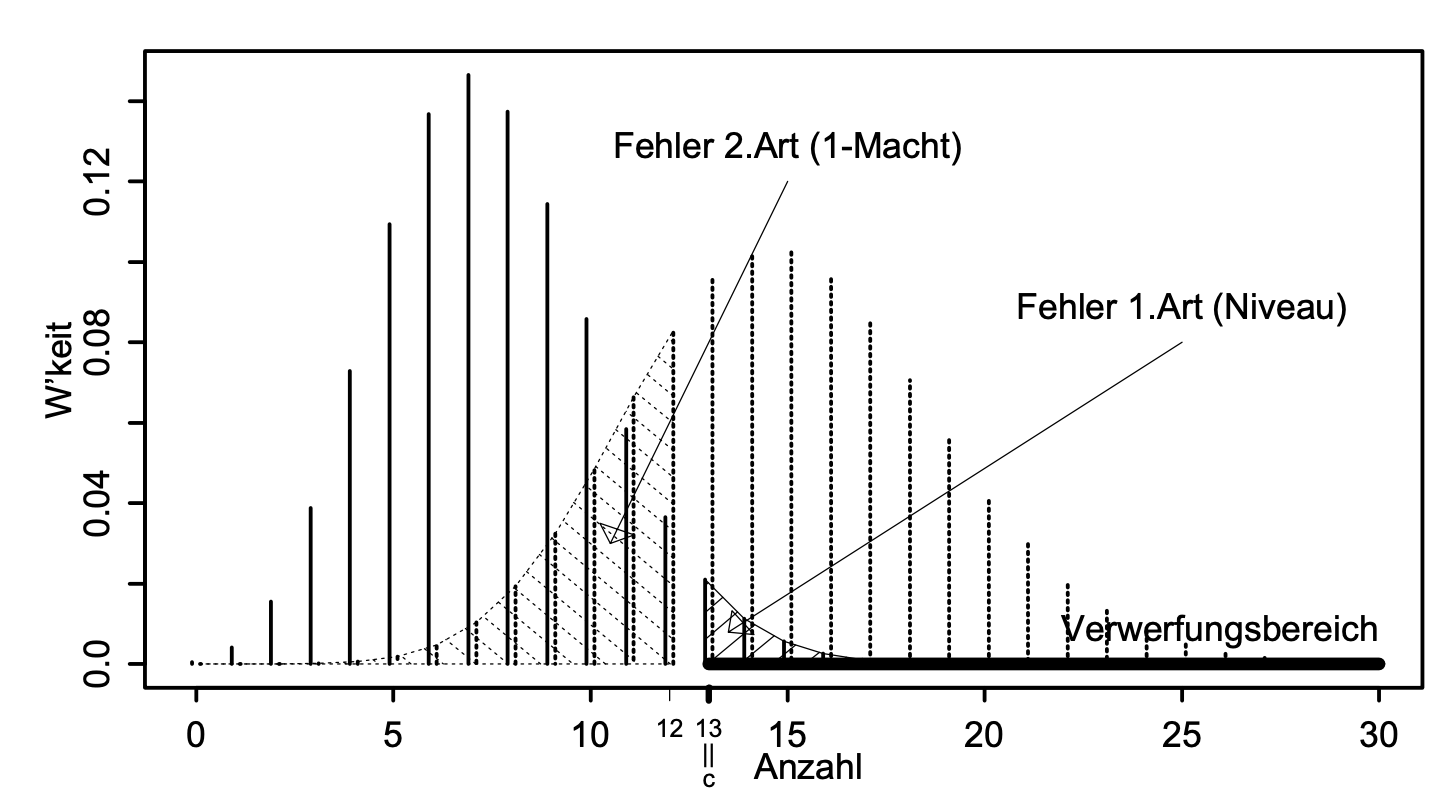
\includegraphics[width=.8\textwidth]{images/normal.png}

\subsection{Begriffe}

Modell: z.B. Unter $P_\varphi$ sind die $X_i$ i.i.d. $\sim\text{Poi}(\lambda)$, $i=1, ..., 6$, $\lambda$ unbekannt.

Teststatistik: Hilfsfunktion bei statistischen Tests. Kann zum Beispiel mittels Likelihood-Quotienten-Vorgehen gefunden werden.


\begin{itemize}
	\item Modell
	\item Nullhypothese
	\item Alternativhypothese
	\item Teststatistik
	\item Verteilung der Teststatistik unter der Nullhypothese
	\item Verwerfungsbereich
	\item beobachteter Wert der Teststatistik
	\item Testentscheid
	\item eventuell $p$-Wert
\end{itemize}

\textbf{Wichtig:}

Falls beobachtetes Ergebnis im Verwerfungsbereich: $H_0$ wird abgelehnt, $H_A$ wird angenommen.

Falls beobachtetes Ergebnis nicht im Verwerfungsbereich: $H_0$ wird nicht abgelehnt (keine Aussage über Annahme!), keine Aussage über $H_A$\\


\textbf{$p$-Wert}: kleinstes Niveau, auf dem der Test die Nullhypothese noch verwirft.\\

Auch: Falls $H_0: p = 123$, $H_A: p < 123$ Mit Statistik $P_{H_0}[T\leq \text{Beobachteter Wert}]$. p-Wert ist so wie die Signifikanz des Testresultats.\\

A small p-value (typically $\leq 0.05$) indicates strong evidence against the null hypothesis, so you reject the null hypothesis.\\

A large p-value ($> 0.05$) indicates weak evidence against the null hypothesis, so you fail to reject the null hypothesis.

\section{Beispiel Teststatistik mit Likelihood-Quotienten finden}

$X_i \sim \text{Poi}(\lambda)$ 

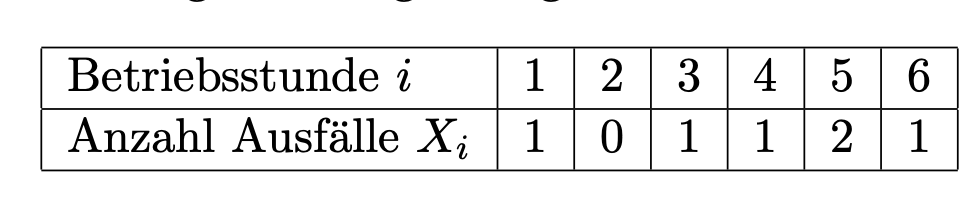
\includegraphics[width=.4\textwidth]{images/likelihood1}

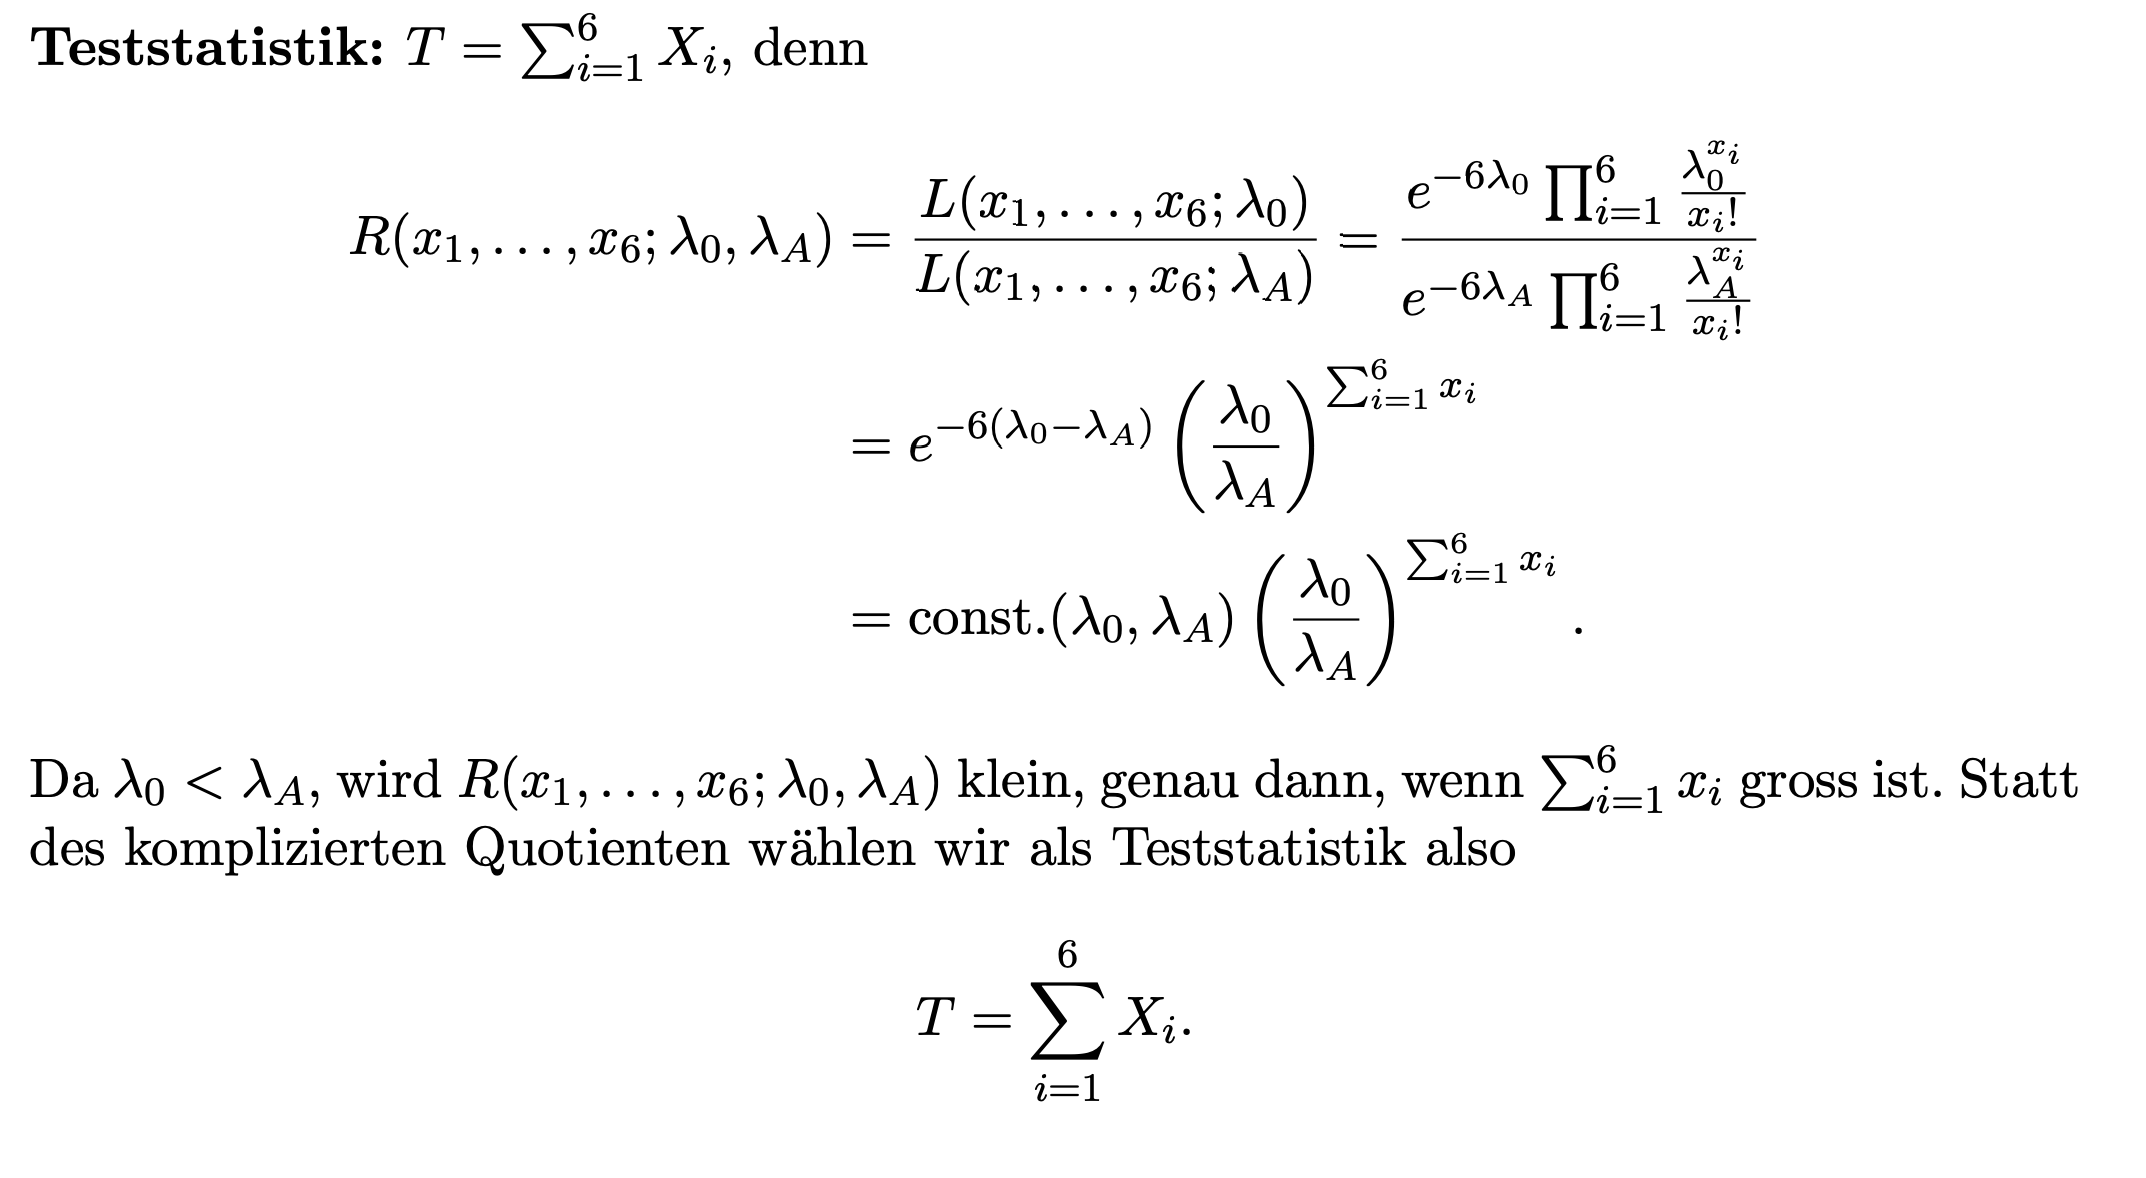
\includegraphics[width=\textwidth]{images/likelihood2}

\section{Konfidenzintervall berechnen}


\begin{itemize}
	\item Gegeben: Teststatistik $T$.
	\item Schätze $\vartheta$ mit einem Schätzer. Zum Beispiel $\mu$: Stichprobenmittel oder $\sigma$: Stichprobenvarianz.
	\item Setze den geschätzten Wert von $\vartheta$ in $T$ ein und bestimme die Verteilung. Achtung: Die Zufallsvariable ist frei. 
	\item Konfidenzintervall mit Niveau $1-\alpha$: Bereich in der neuen Verteilung, die die Fläche $1-\alpha$ hat. ACHTUNG: Bereich soll als Bereich der Zufallsvariable angegeben sein, bevor sie in die Teststatistik eingeben wird, sodass sie im Niveaubereich liegt.
\end{itemize}













































%\section{Einfache Lineare Regression}
Wir betrachten lediglich zwei Zufallsvariablen $X,Y$, zwischen denen wir einen linaren Zusammenhang vermuten. Dies schreiben wir durch ein Modell der Form
$$ Y = \beta_0 + \beta_1 X + \varepsilon$$
für konstante $\beta_0,\beta_1$ und eine von $X$ unabhängige Zufallsvariable $\varepsilon$ mit $\E[\varepsilon] = 0$ und endlicher Varianz.\\

Seien $(x_i, y_i)$ für $i \in \{1,\dots,n\}$ unabhängige Realisierungen von $(X,Y)$, also von uns beobachtete Daten. Wir suchen die Paramter $\beta_0,\beta_1$ mittels der Methode der kleinsten Quadrate, d.h. wir minimieren
$$ f(\beta_0, \beta_1) := \sum_{i=1}^n (\beta_0 + \beta_1 x_i - y_i)^2$$
in dem wir nach $\beta_0$ und $\beta_1$ ableiten, und den Gradient $\nabla f=0$ setzen. Zuerst definieren wir aber 
$$ \overline{x}:= \frac{1}{n}\sum_{i=1}^n x_i, \quad \quad \overline{y}:= \frac{1}{n}\sum_{i=1}^n y_i, \quad \quad \overline{x^2}:= \frac{1}{n}\sum_{i=1}^n x_i^2, \quad \quad \overline{xy}:= \frac{1}{n}\sum_{i=1}^n x_i y_i$$
Nun finden wir den Gradienten von $f$ und setzen ihn $=0$: 
$$ \nabla f(\beta_0, \beta_1) = \begin{pmatrix}
2 \sum_{i=1}^n (\beta_0 + \beta_1 x_i - y_i) \\ 
2 \sum_{i=1}^n x_i ( \beta_0 + \beta_1 x_i - y_i)
\end{pmatrix} \overset{!}{=} 0 \implies \beta_0 + \beta_1 \overline{x} = \overline{y} \quad \land \quad \beta_0 \overline{x}  + \beta_1 \overline{x^2} = \overline{xy}$$
Dieses Gleichungssystem kann man nun auflösen und erhält:
\begin{mdframed}[backgroundcolor=red!20]
$$ \beta_1 = \frac{\mathrm{cov}(x,y)}{\mathrm{var}(x)} \quad \quad \quad \quad \quad  \beta_0 = \overline{y} - \frac{\mathrm{cov}(x,y)}{\mathrm{var}(x)}\overline{x} $$
\end{mdframed}
wobei $\mathrm{var}(x)$ und $\mathrm{cov}(x,y)$ die \textit{Stichprobenvarianz} bzw. \textit{Strichprobenkovarianz} bezeichnet. Beachte, dass diese Schätzungen nicht erwartungstreu sind, und man deshalb oft die korrigierten Varianten benutzt:
\begin{eqnarray*}
\mathrm{var}(x) := \frac{1}{n}\sum_{i=1}^n (x_i - \overline{x})^2 & \mbox{ vs. } & \frac{1}{n-1} \sum_{i=1}^n (x_i - \overline{x})^2 \\
\mathrm{cov}(x,y) := \frac{1}{n} \sum_{i=1}^n (x_i - \overline{x})(y_i - \overline{y}) & \mbox{ vs. } & \frac{1}{n-1} \sum_{i=1}^n (x_i - \overline{x})(y_i - \overline{y})
\end{eqnarray*}
Für grosse $n$ wird dieser Unterschied jedoch zunehmened geringer und es spielt dann keine Rolle mehr, welche Formel verwendet wird.



% fill the page
%\clearpage

%\end{multicols}

\end{document}


